\chapter{SYSTEM DESIGN}
\label{chap:system_design}

This chapter breaks down SmartExam's technical architecture, converting our requirements into a functional design by defining database schema, component structure diagrams, and runtime diagrams. This diagram set serves as our blueprint to guide WPF client, API controllers, WebSocket hub, and grading service communication when under stress.

\section{Structure Diagrams}
Structure diagrams display a system's compile-time structure, which we apply to diagramming our database model, server processes and client applications \cite{structure_diagram_techopedia}. These help to determine compile-time bounds and enable parallel development among team members by revealing how components will fit together.

When designing SmartExam's overall architecture, structure diagrams assist by visually identifying how the database models, controllers, servers and clients relate and connect. This visual diagram helps to clarify our application's static foundation, including how to manage authentication, how to establish lockdown limits and what order in which we would like to perform gradings.

\subsection{Class Diagram}
In our system design, we use class diagrams to depict the database entity-relationship diagram (ERD) that define our application's data structure as object classes \cite{class_diagram_uml, class_diagram_sparx}. We've represented some core models here in Figure~\ref{fig:class_diagram}.

\begin{figure}[H]
\centering
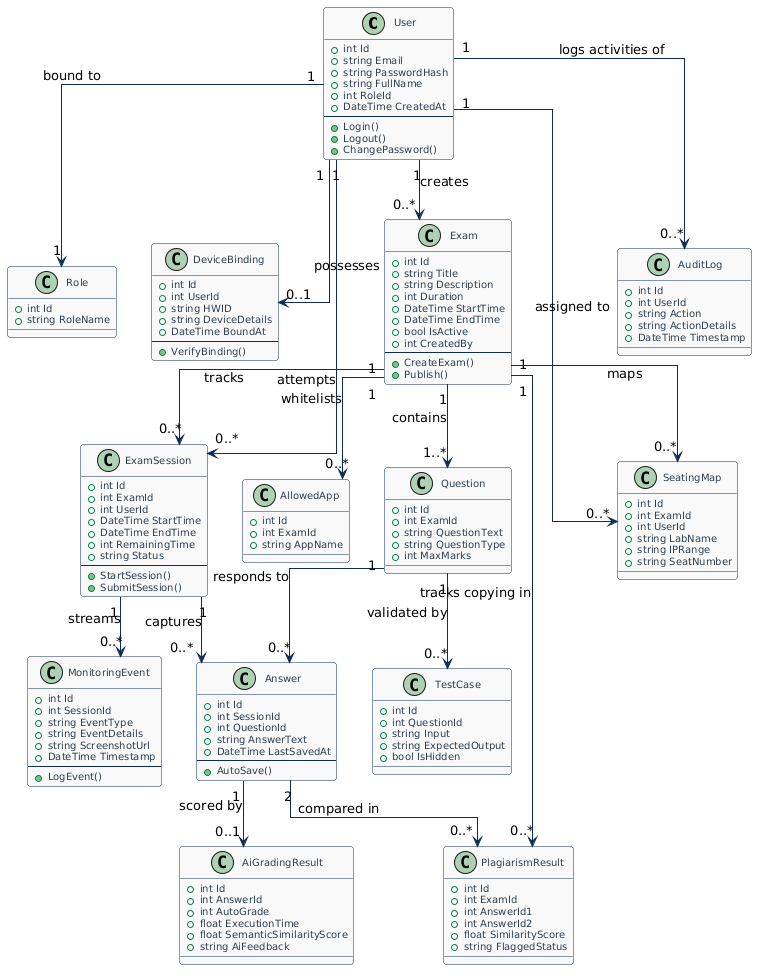
\includegraphics[width=0.97\linewidth]{Figures/class_diagram.png}
\caption{UML Class Diagram of the SmartExam Object Model}
\label{fig:class_diagram}
\end{figure}

The fourteen classes represented in Figure~\ref{fig:class_diagram} illustrate the attributes of our 14 essential database entities. Here we model our 14 database entities, which are roles, user profiles, HW (hardware ID) bindings, settings, exam settings, seating plans, telematics events and exam log files. Note how the two entities with a 1:1 relationship between them represent binding an exam setting with user. This would give our security team more control over which machines and OSes exams are allowed on, blocking students taking exams on their personal devices or a non-proctored machine.

\subsection{Deployment Diagrams}
A Deployment Diagram illustrates the hardware architecture of the deployment target, and displays the software mapping onto hardware and network topology \cite{sequence_diagram_medium}. In this Diagram, we can clearly observe our system architecture, which is set up in the cloud.

\begin{figure}[H]
\centering
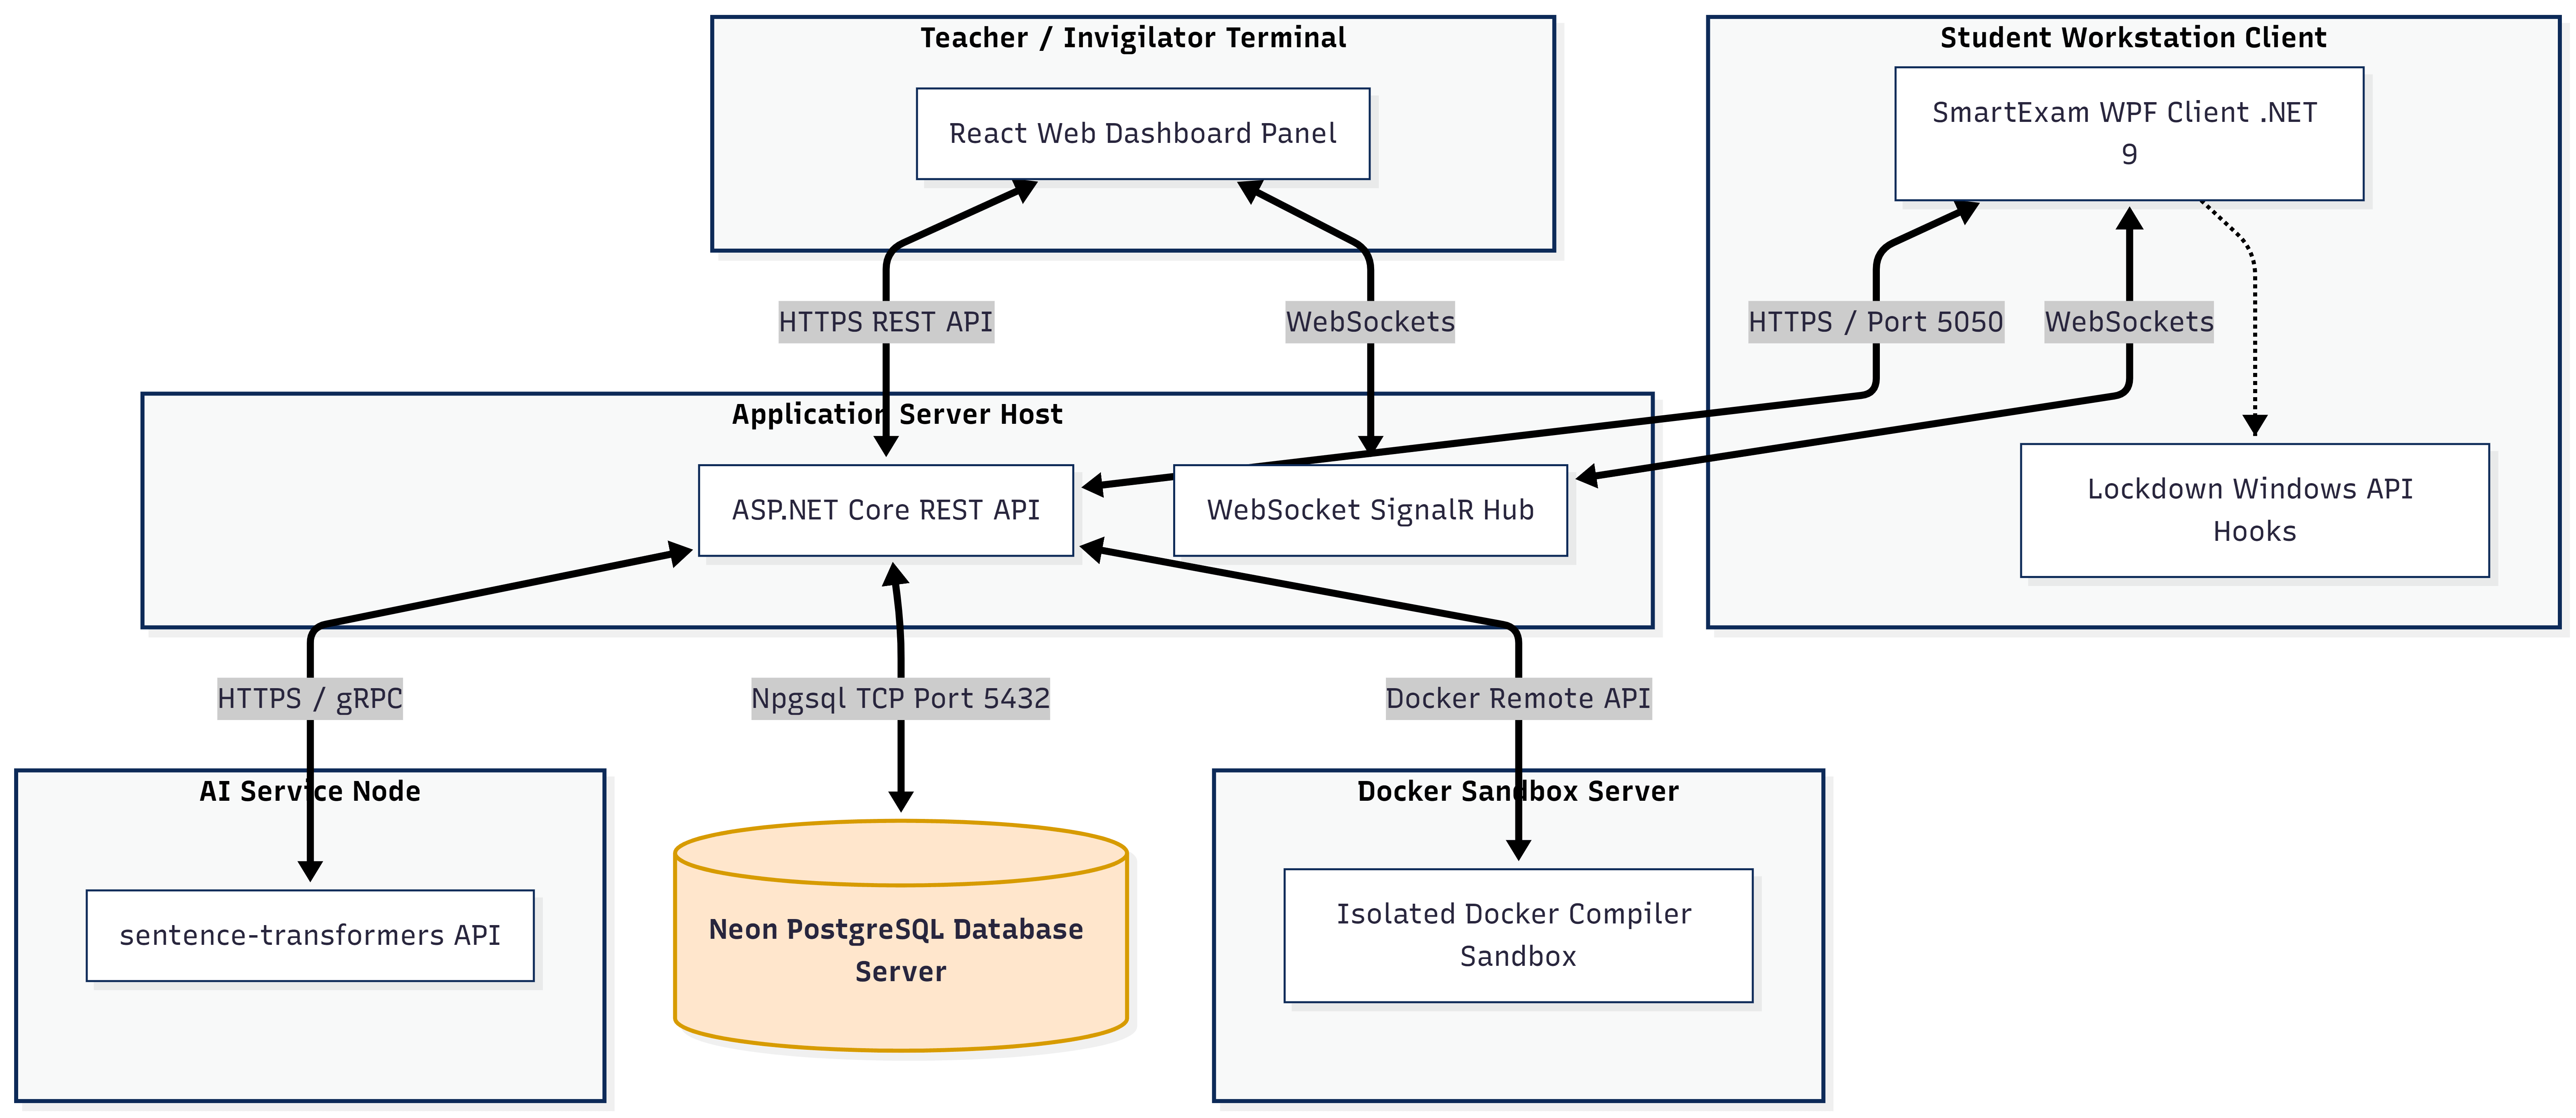
\includegraphics[width=0.97\linewidth]{Figures/deployment_diagram.png}
\caption{UML Deployment Diagram of the SmartExam Distributed Topology}
\label{fig:deployment_diagram}
\end{figure}

As shown in Figure~\ref{fig:deployment_diagram}, we divide our platform into three physical tiers. The Client tier contains the WPF student client running locally. The Web tier serves the React admin panel to teachers. The Server tier hosts the ASP.NET Core API server, which communicates with Neon PostgreSQL, a sandboxed Docker execution host, and our AI semantic grading microservice. Communication uses HTTPS for REST endpoints and WebSockets for real-time telemetry.

\subsection{Component Diagram}
Component diagrams detail the modular interfaces and dependencies of our compile-time blocks. Figure~\ref{fig:component_diagram} shows how they connect.

\begin{figure}[H]
\centering
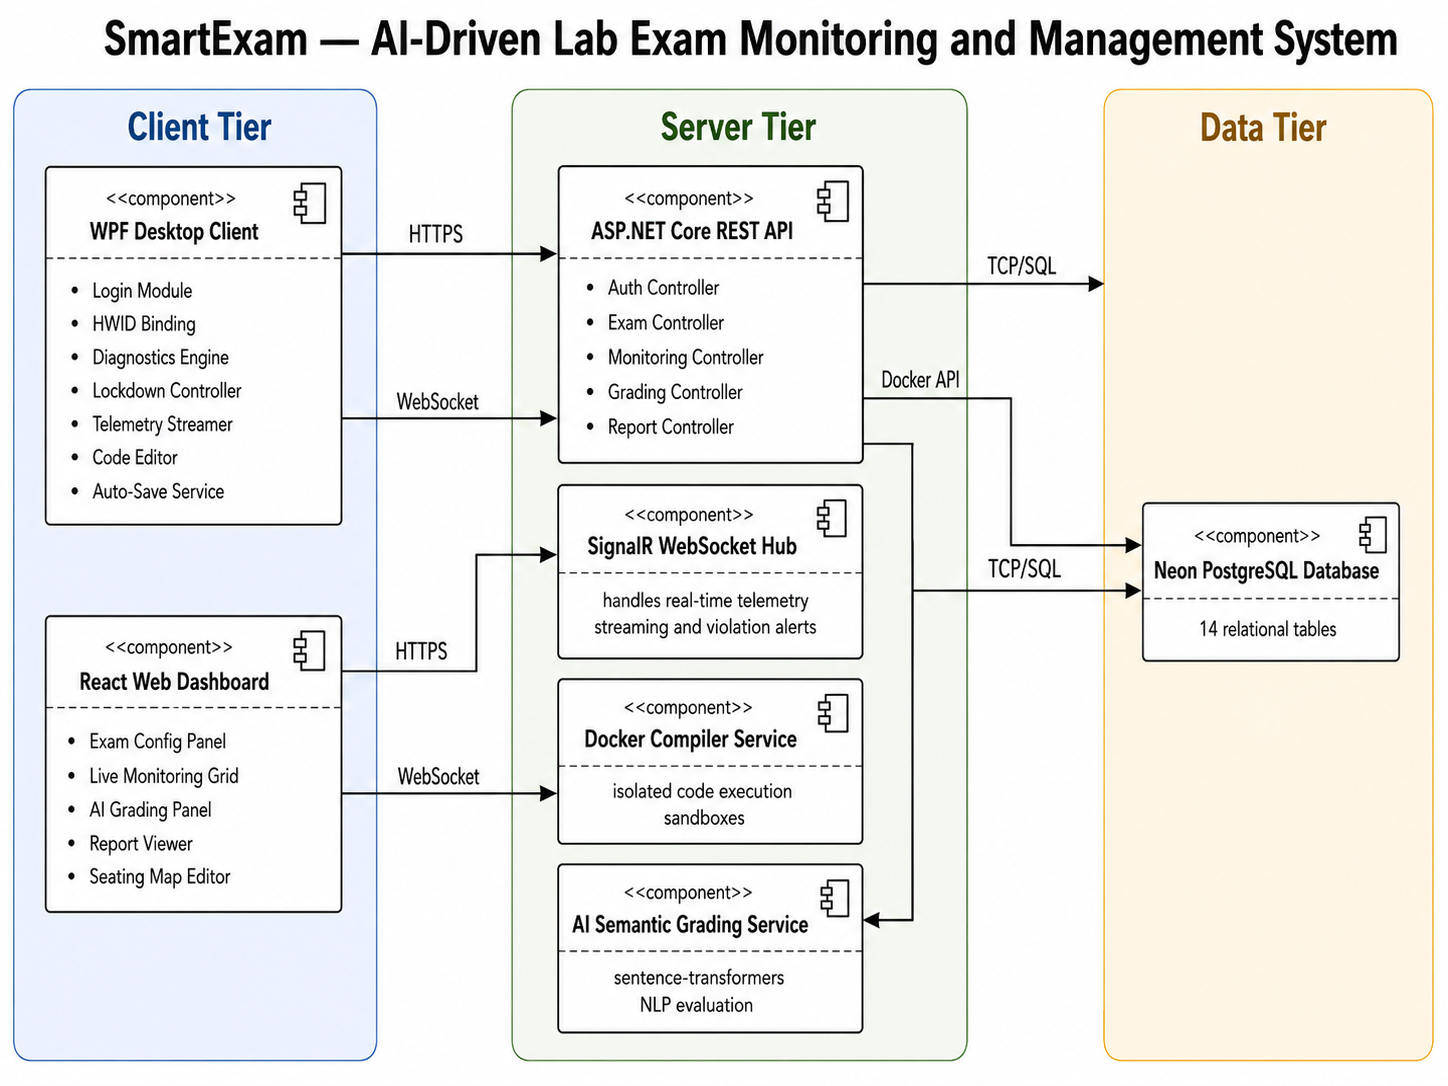
\includegraphics[width=0.97\linewidth]{Figures/component_diagram.png}
\caption{UML Component Diagram of the SmartExam System Architecture}
\label{fig:component_diagram}
\end{figure}

In Figure~\ref{fig:component_diagram}, we separate the system into Client, Application, and Data tiers. The WPF and React components make up the client tier. The REST API, SignalR WebSockets hub, Docker grading runner, and AI semantic parser run in the application tier. The Neon PostgreSQL database holds our persistent storage.

\section{Behavioral Diagrams}
Behavioral diagrams represent how the components of our systems interact during the execution time. These types of diagrams illustrate how data flows through the system and provide a step by step walk through as certain actions occur such as the change in state or other system events occur \cite{behavioral_uml_diagrams}.

\subsection{Activity Diagrams}
In computer science, an activity diagram is a flow chart like diagram which will be the diagram used to show each step that leads up to a part of a workflow, which will in turn, be one step in another, higher level workflow \cite{activity_diagram_vp}. The student exam section, and the lockdown workflow are two of our most common workflows depicted below.

\subsubsection{Student Exam Session and Lockdown Workflow}
The Diagram below in Figure~\ref{fig:activity_diagram} summarizes the typical exam workflow taken by our student application, all the way from logging in to submitting his answers. From authentication and the submission to the HWID Check the student will log into their workstation and get the signal to proceed to lockdown where local diagnostics take place. Before they even click on the ``start exam'' button the system has already initiated screenshot and focus polling, ready for anything out of the normal.

\begin{figure}[H]
\centering
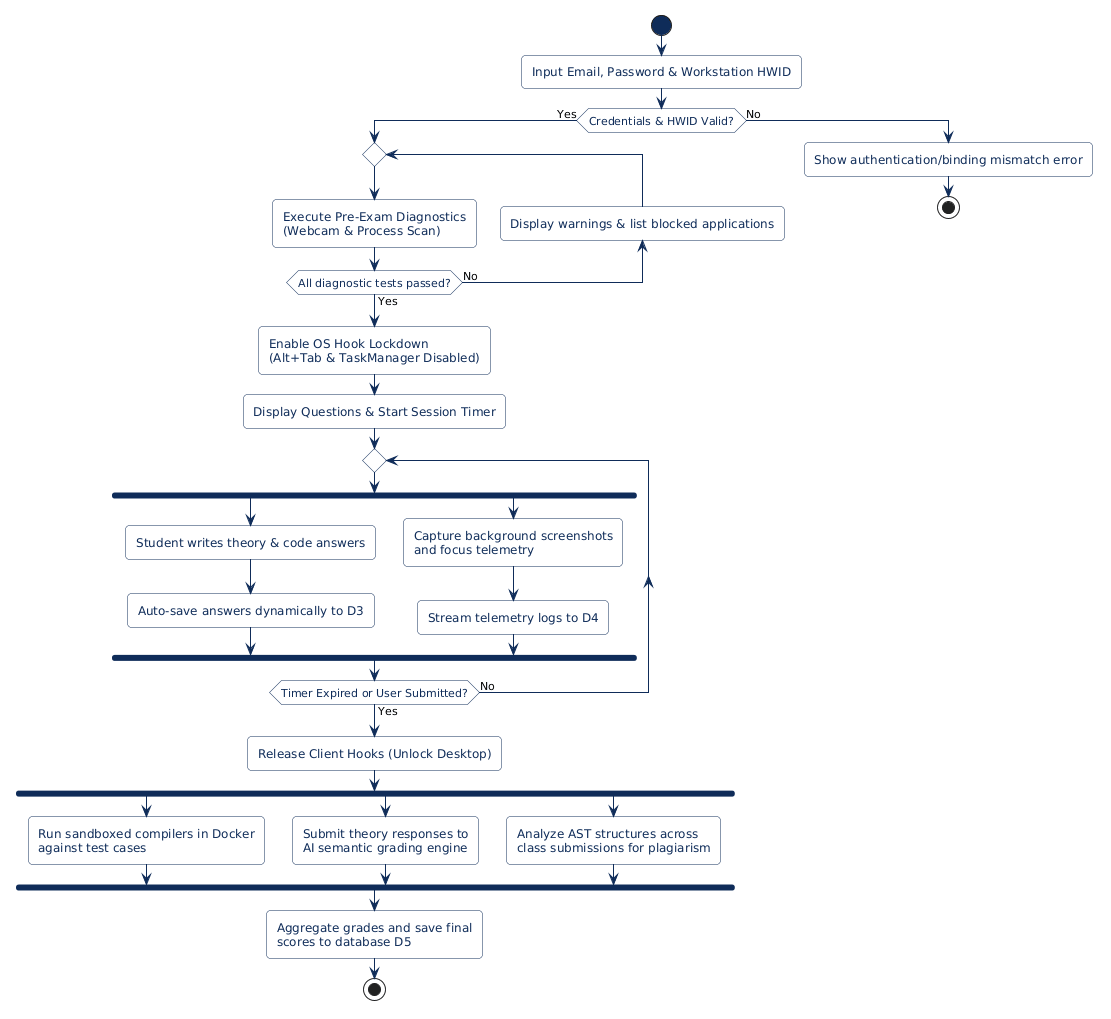
\includegraphics[width=0.97\linewidth]{Figures/activity_diagram.png}
\caption{UML Activity Diagram of Student Exam Session and Lockdown Workflow}
\label{fig:activity_diagram}
\end{figure}

\subsubsection{Authentication and HWID Binding}
Figure~\ref{fig:activity_auth} maps the workstation binding checks.

\begin{figure}[H]
\centering
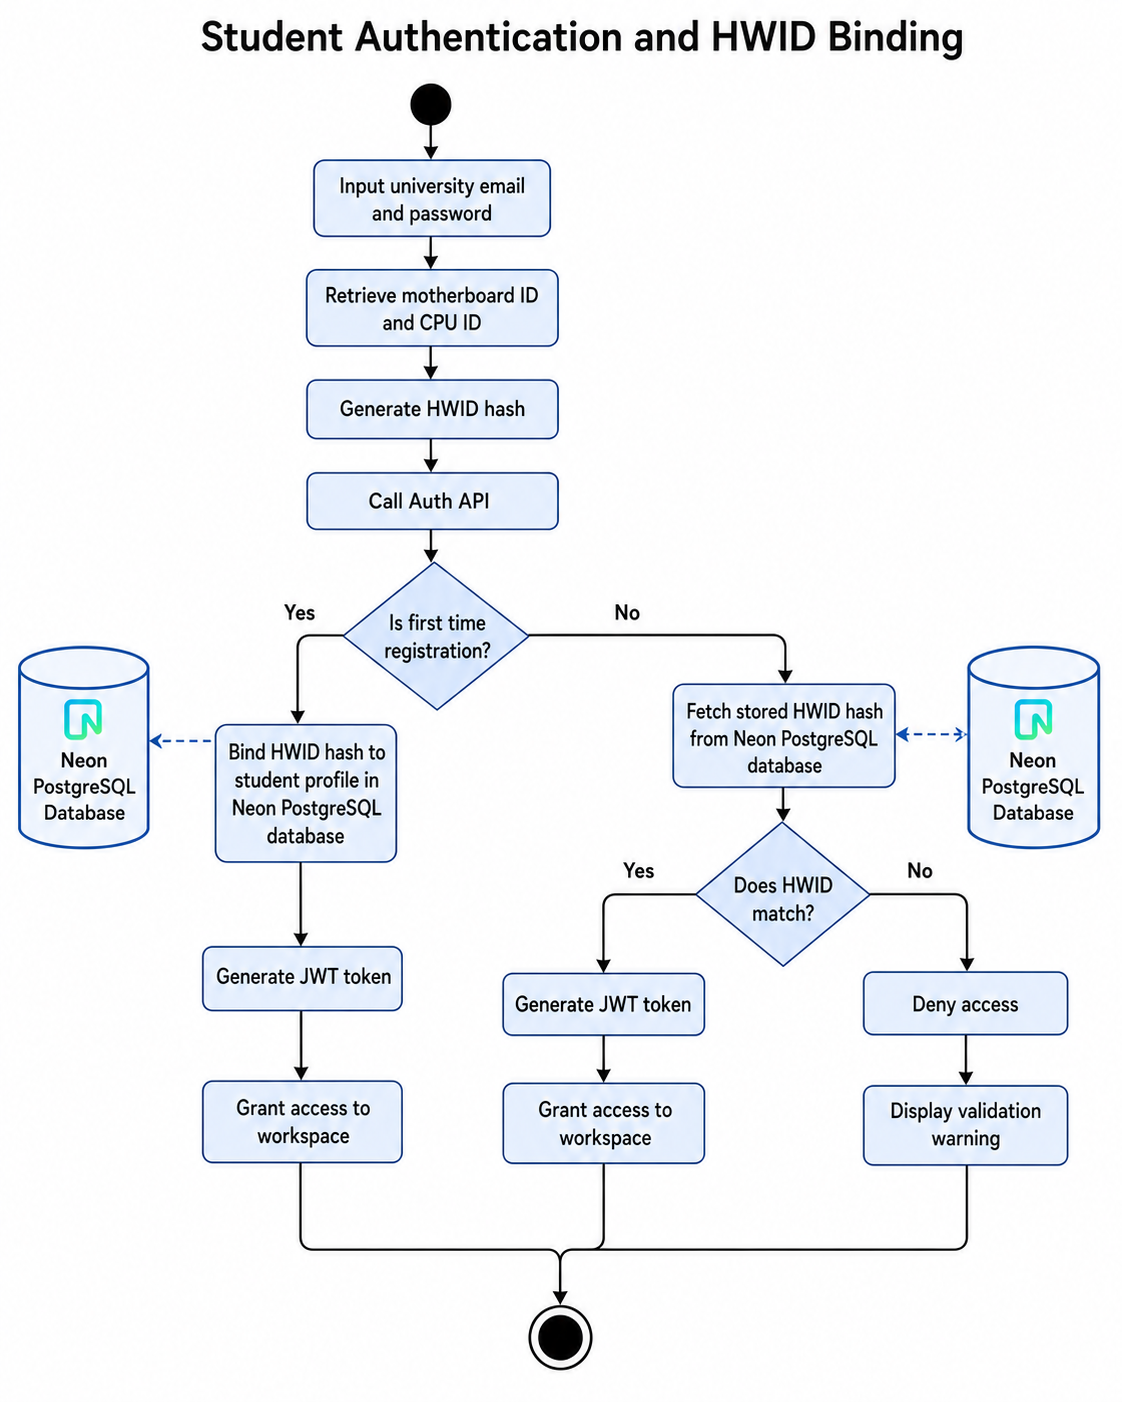
\includegraphics[width=0.97\linewidth]{Figures/activity_auth.png}
\caption{UML Activity Diagram of Student Authentication and HWID Binding}
\label{fig:activity_auth}
\end{figure}

Our diagram of the authentication and HWID Check is included here below for clarity and for demonstrating the role of security in the exam workflow. Once the system has performed initial client/server authentications the system may retrieve and store the initial CPU and motherboard serial hashes for that workstation. The first time a student logs into a workstation, that binding will be recorded in our server-side database. The following attempts to log in to that workstation by that student will require that the server-side binding hashes must match the client-side.

\subsubsection{Pre-Exam Diagnostics Check}
Figure~\ref{fig:activity_diagnostics} shows the pre-exam verification flow.

\begin{figure}[H]
\centering
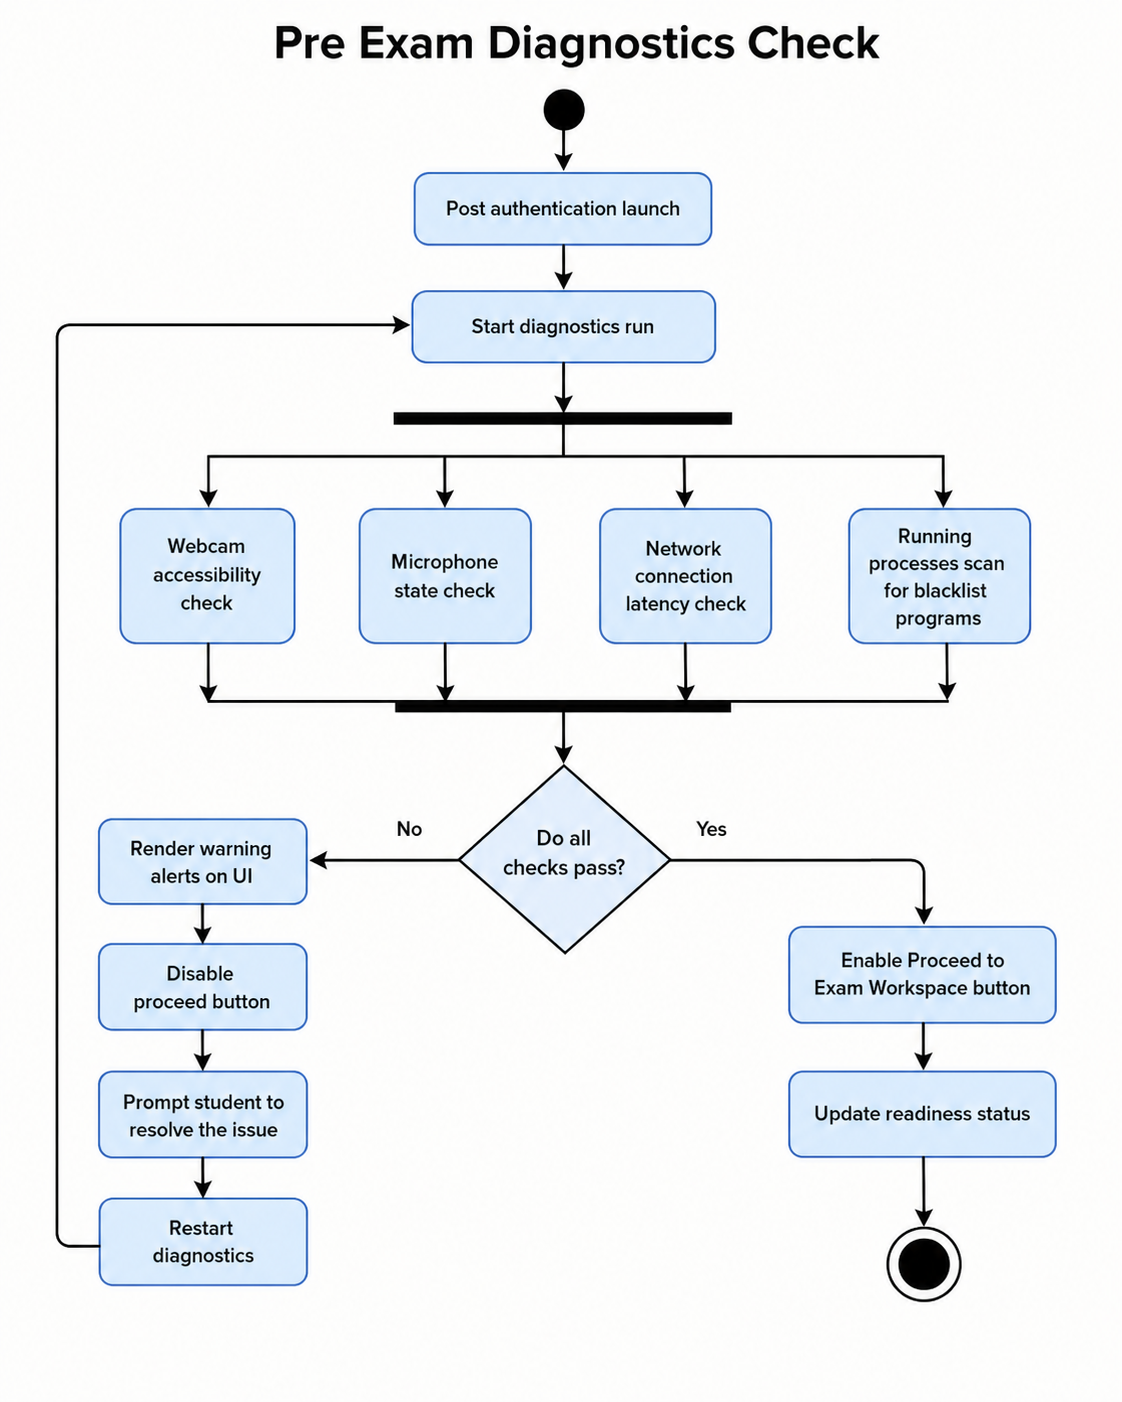
\includegraphics[width=0.97\linewidth]{Figures/activity_diagnostics.png}
\caption{UML Activity Diagram of Pre-Exam Diagnostics Check}
\label{fig:activity_diagnostics}
\end{figure}

This section diagram (Figure~\ref{fig:activity_diagnostics} below) provides details on what will happen before the student is allowed to actually ``start the exam''. Local diagnostic tests for web-cam presence, internet connectivity, and lists of prohibited applications will be performed, and the user will be alerted to any failures.

\subsubsection{Readiness Verification and Mock Test}
Figure~\ref{fig:activity_readiness} outlines the mock test environment.

\begin{figure}[H]
\centering
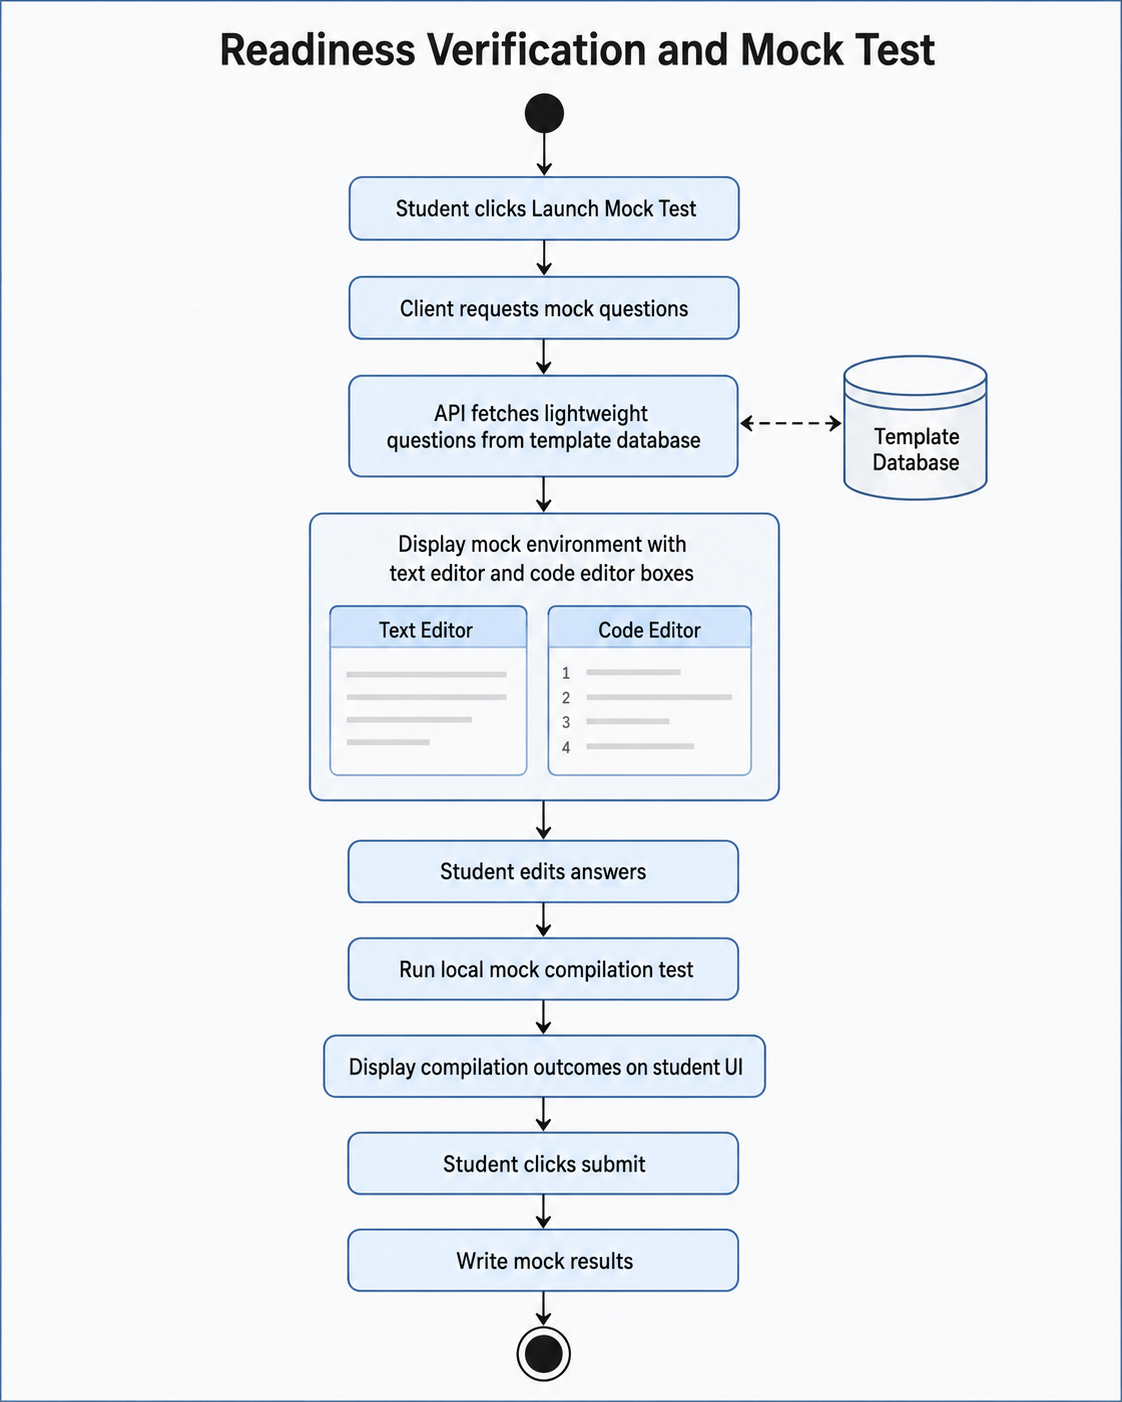
\includegraphics[width=0.97\linewidth]{Figures/activity_readiness.png}
\caption{UML Activity Diagram of Readiness Verification and Mock Test}
\label{fig:activity_readiness}
\end{figure}

The following Diagram (Figure~\ref{fig:activity_readiness}) indicates what is necessary in order to be ``ready'' and what happens before a ``practice'' test would take place. For a practice test, it's expected that the student would have all necessary items in place, and have a clean network connection.

\subsubsection{Active Exam Dashboard}
Figure~\ref{fig:activity_dashboard} shows the active exam dashboard flow.

\begin{figure}[H]
\centering
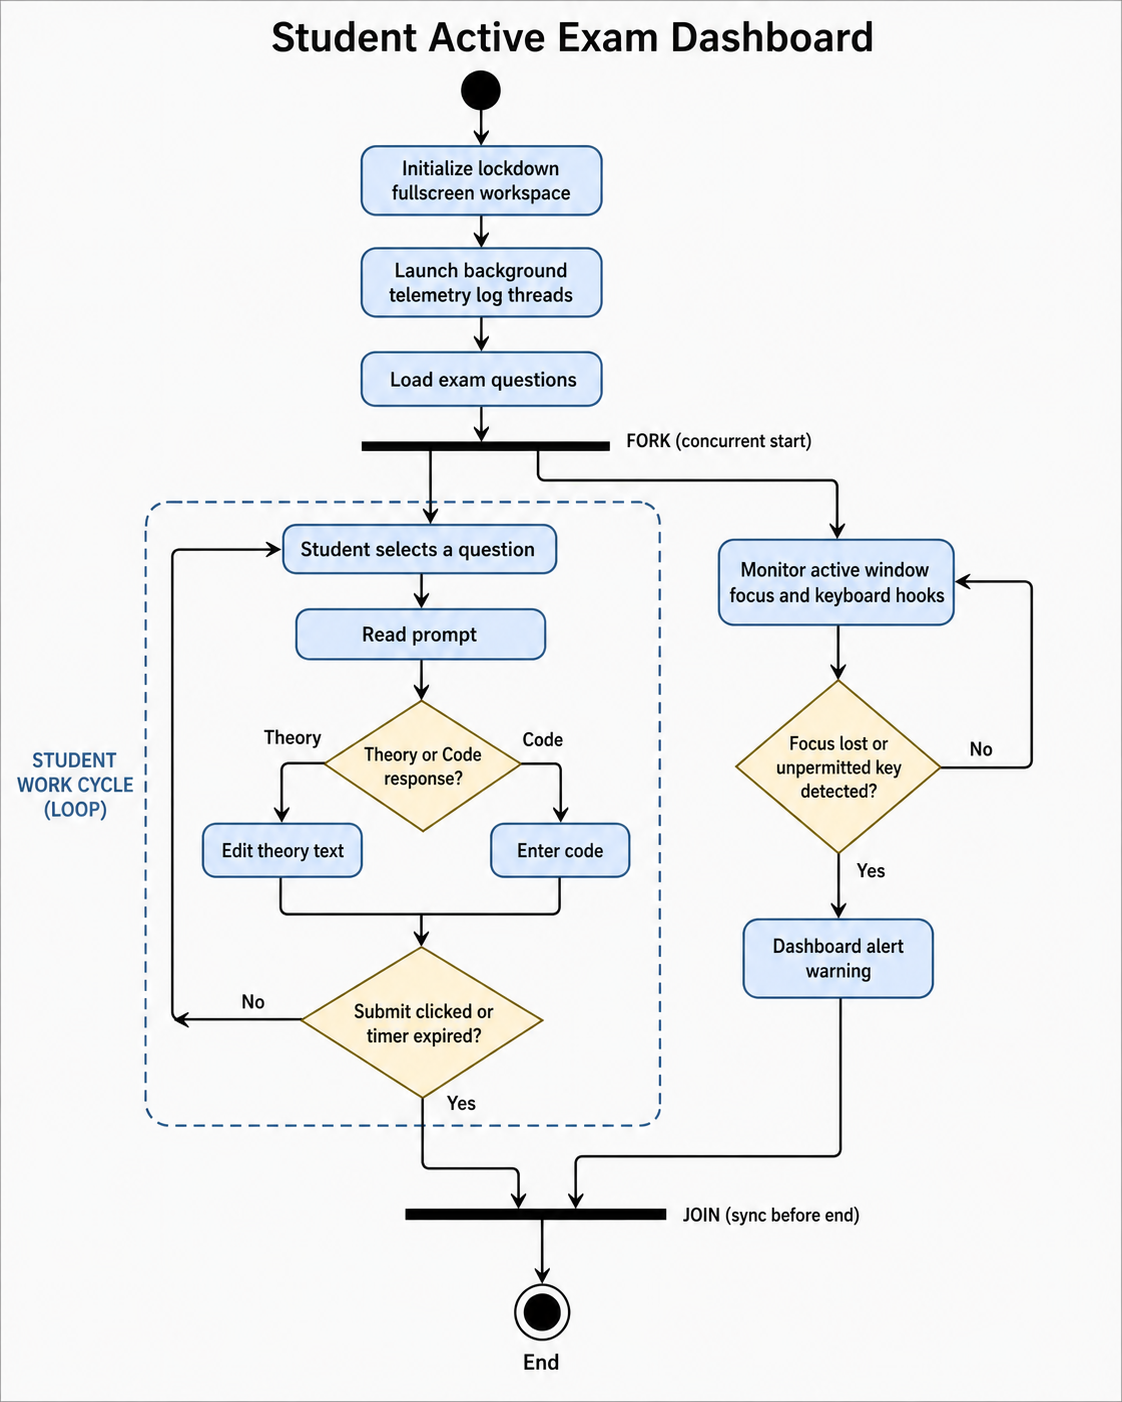
\includegraphics[width=0.97\linewidth]{Figures/activity_dashboard.png}
\caption{UML Activity Diagram of Student Active Exam Dashboard}
\label{fig:activity_dashboard}
\end{figure}

The dashboard enforces full-screen mode, disables desktop hotkeys, and tracks user actions. Students write code or text and submit before the session timer runs out.

\subsubsection{Auto-Save and Session Recovery}
Figure~\ref{fig:activity_recovery} details the auto-save loop.

\begin{figure}[H]
\centering
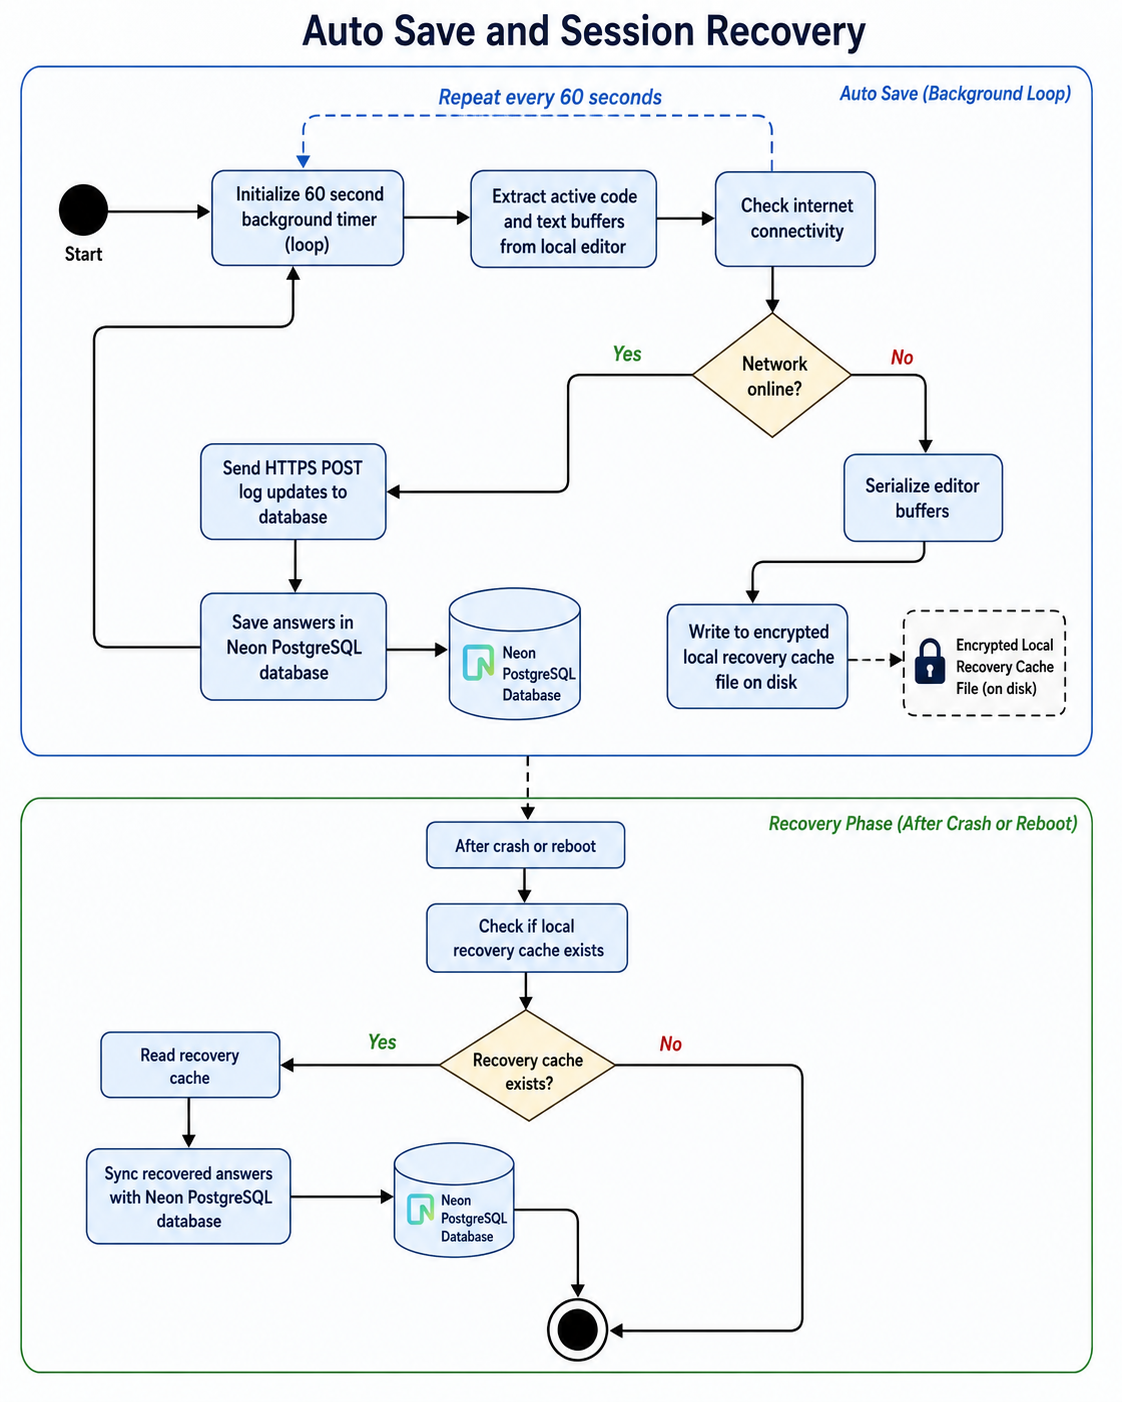
\includegraphics[width=0.97\linewidth]{Figures/activity_recovery.png}
\caption{UML Activity Diagram of Auto-Save and Session Recovery}
\label{fig:activity_recovery}
\end{figure}

A background timer triggers every 60 seconds. If the client is online, it uploads active drafts to the database. If the network drops, it caches the encrypted drafts locally and syncs them once the connection recovers.

\subsubsection{Controlled Exam Submission}
Figure~\ref{fig:activity_submission} shows the submission pipeline.

\begin{figure}[H]
\centering
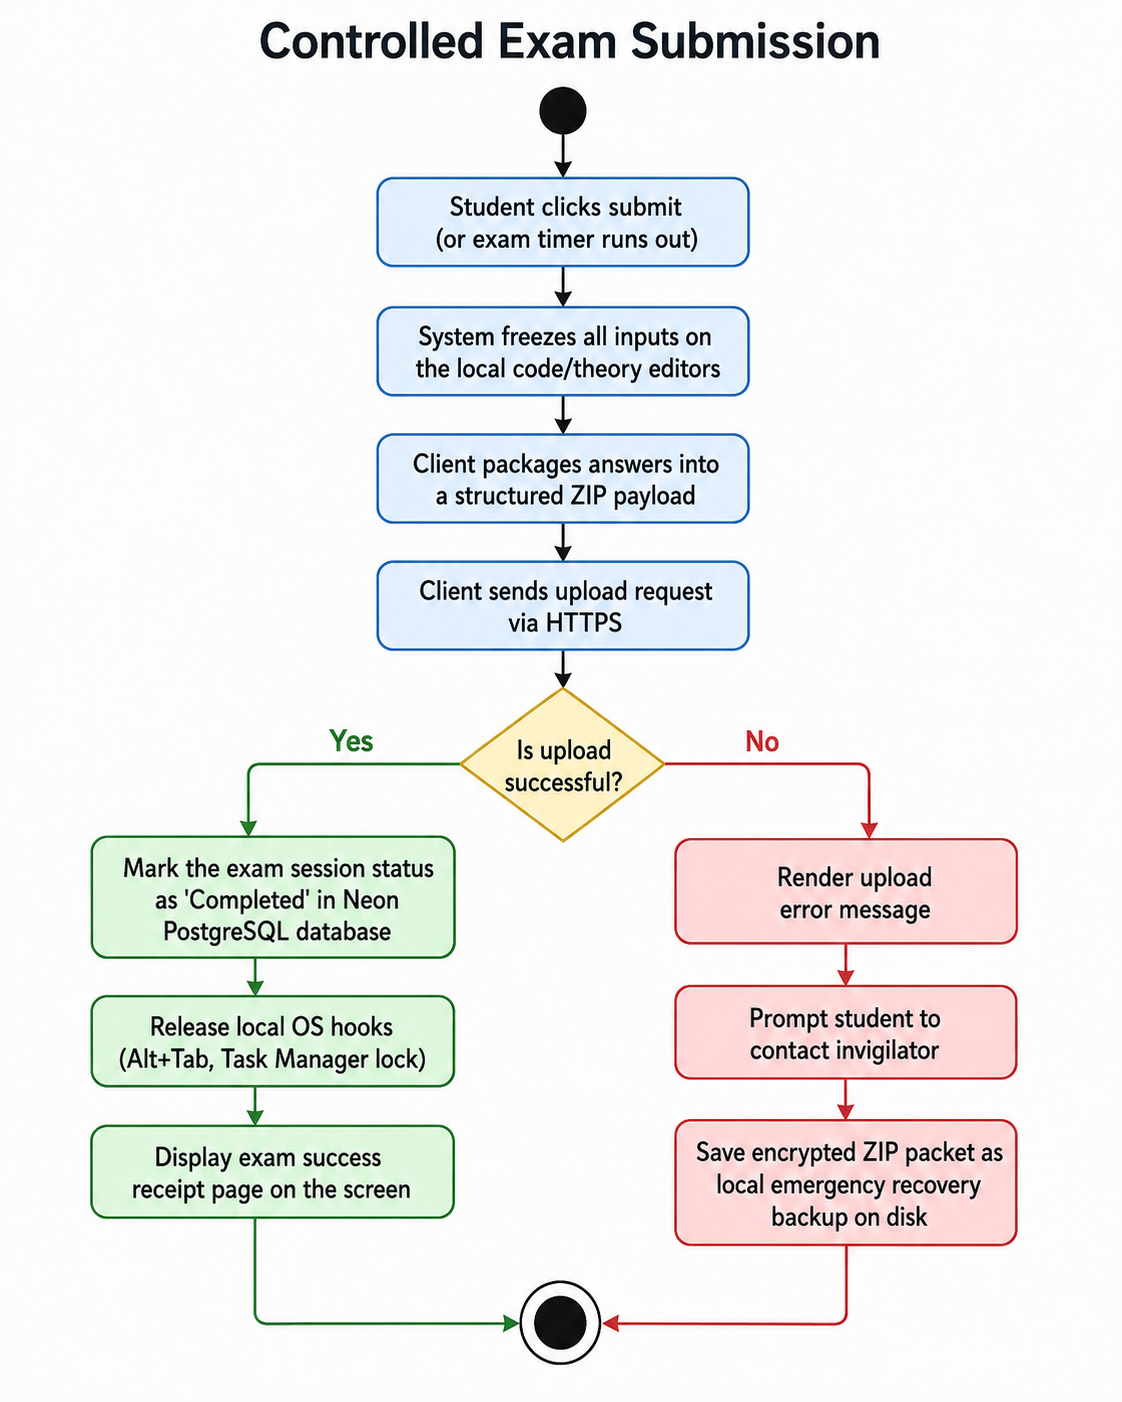
\includegraphics[width=0.97\linewidth]{Figures/activity_submission.png}
\caption{UML Activity Diagram of Controlled Exam Submission}
\label{fig:activity_submission}
\end{figure}

When submitting, the client packages files, uploads them over HTTPS, registers the completion event in the database, removes all key hooks, and exits. 

\subsubsection{Exam Template Configuration}
Figure~\ref{fig:activity_config} maps how teachers configure exams.

\begin{figure}[H]
\centering
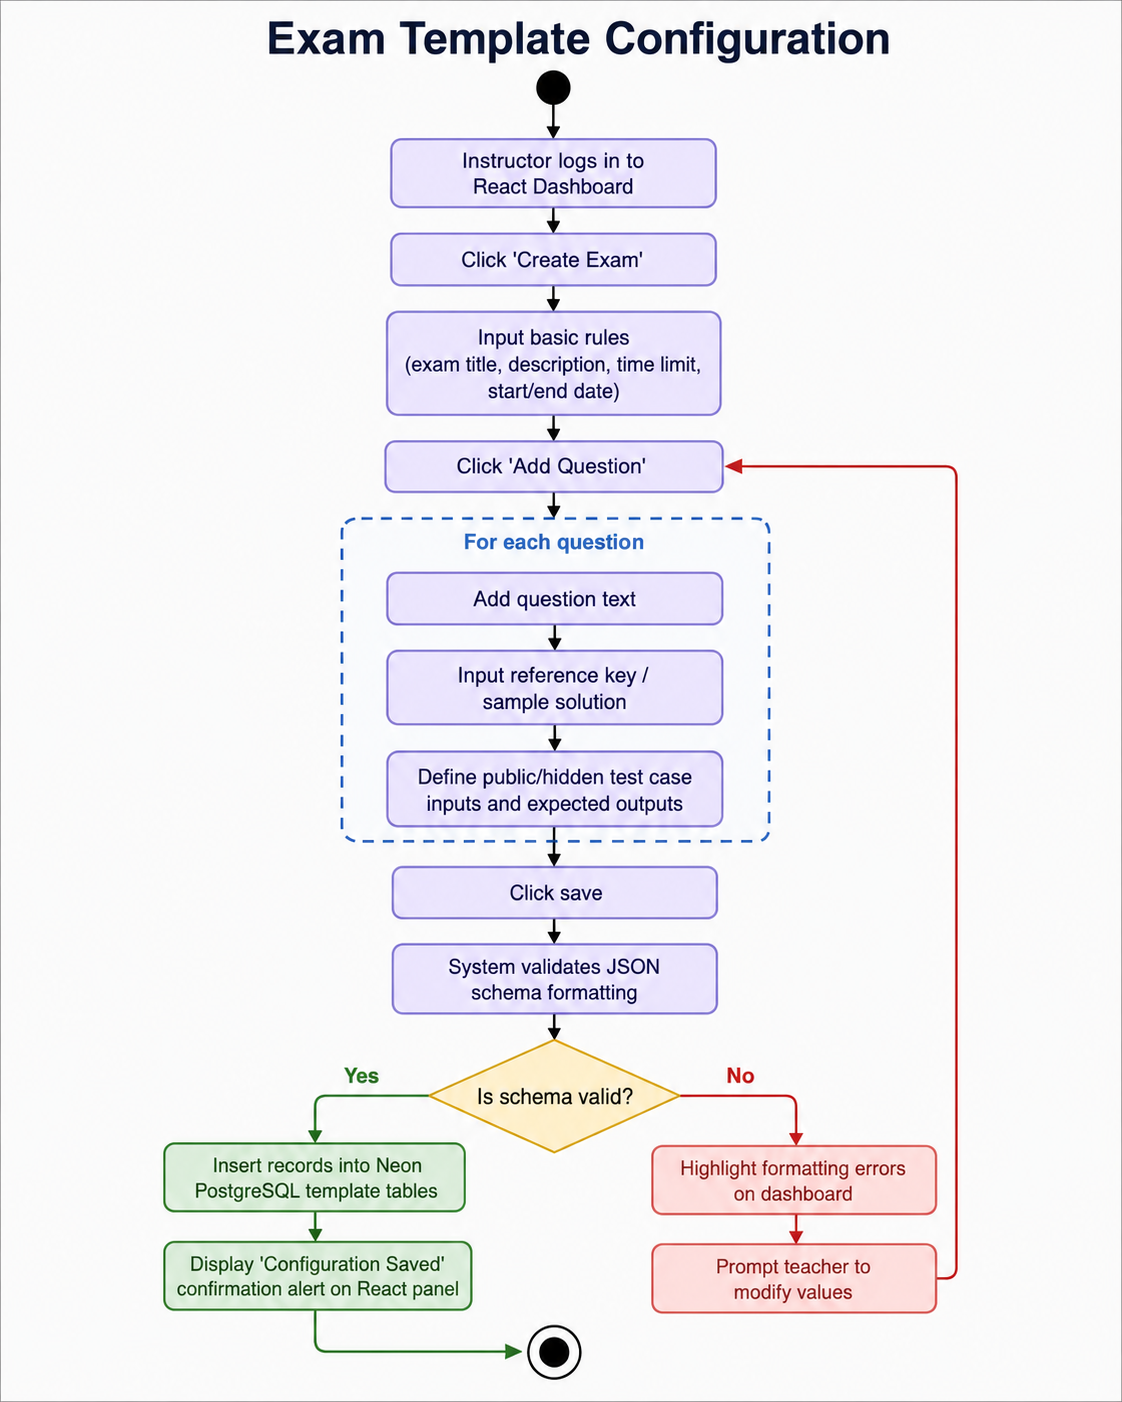
\includegraphics[width=0.97\linewidth]{Figures/activity_config.png}
\caption{UML Activity Diagram of Exam Template Configuration}
\label{fig:activity_config}
\end{figure}

Teachers configure questions, assign weights, define test cases, and save settings to the database.

\subsubsection{Allowed Applications Configuration}
Figure~\ref{fig:activity_applications} shows whitelisting.

\begin{figure}[H]
\centering
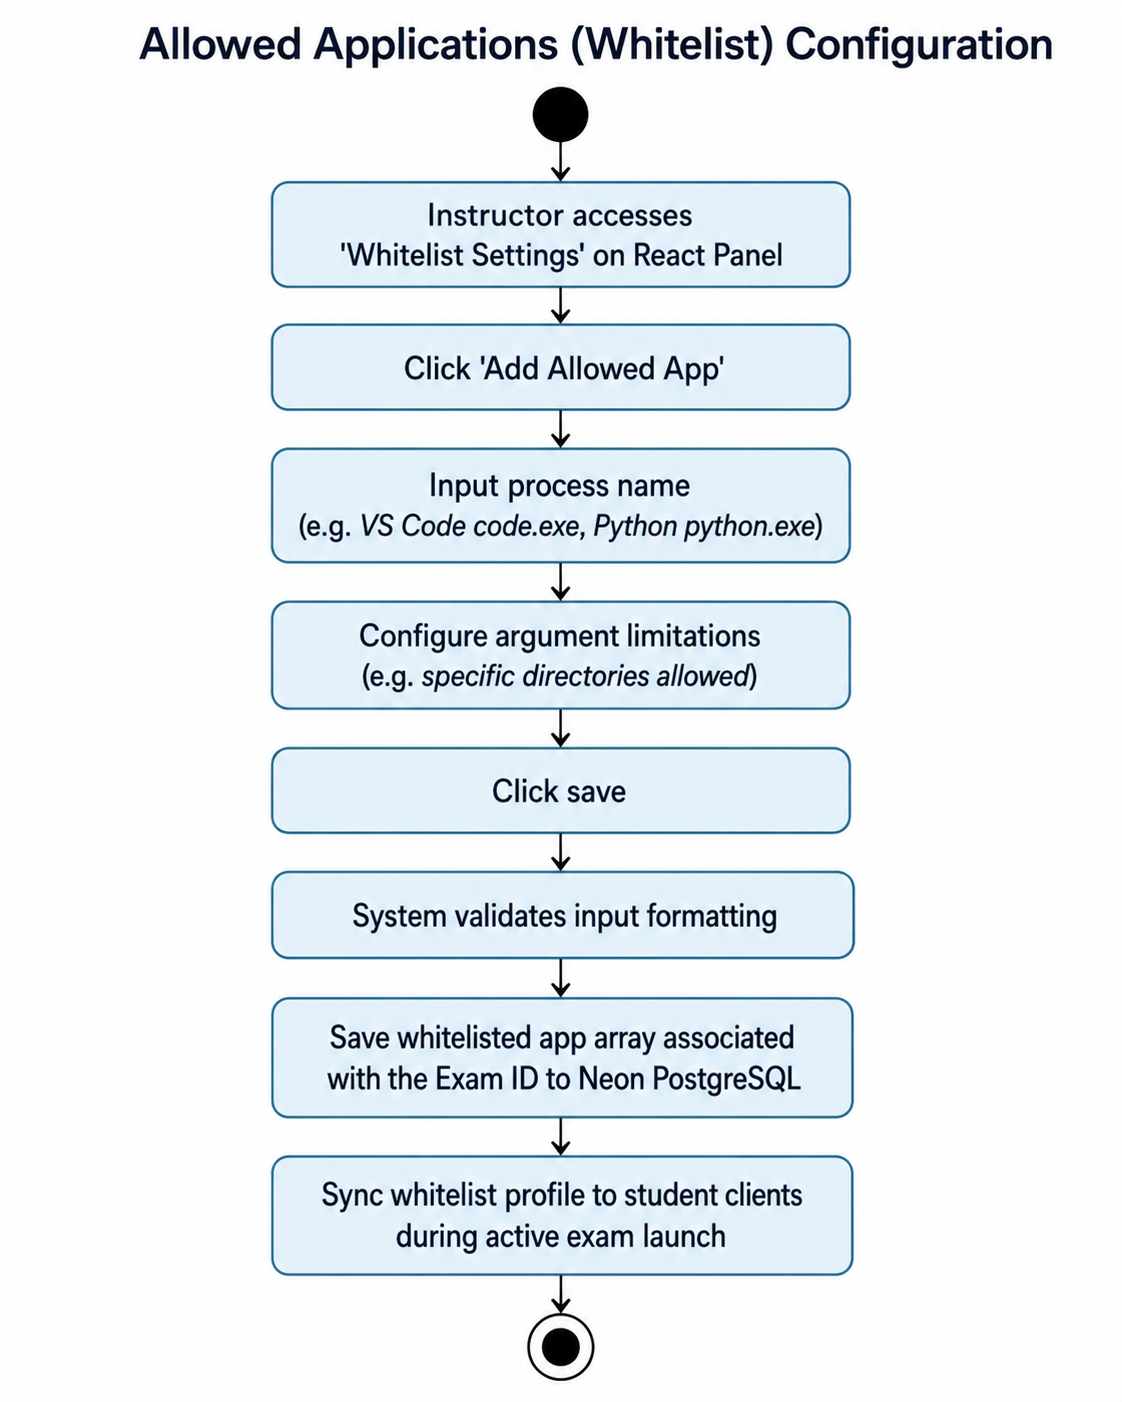
\includegraphics[width=0.97\linewidth]{Figures/activity_applications.png}
\caption{UML Activity Diagram of Whitelisted Applications Configuration}
\label{fig:activity_applications}
\end{figure}

Teachers select allowed executables (e.g., \texttt{code.exe}) and save the list to define lockdown boundaries.

\subsubsection{Access Control and Seating Mapping}
Figure~\ref{fig:activity_seating} details seating maps.

\begin{figure}[H]
\centering
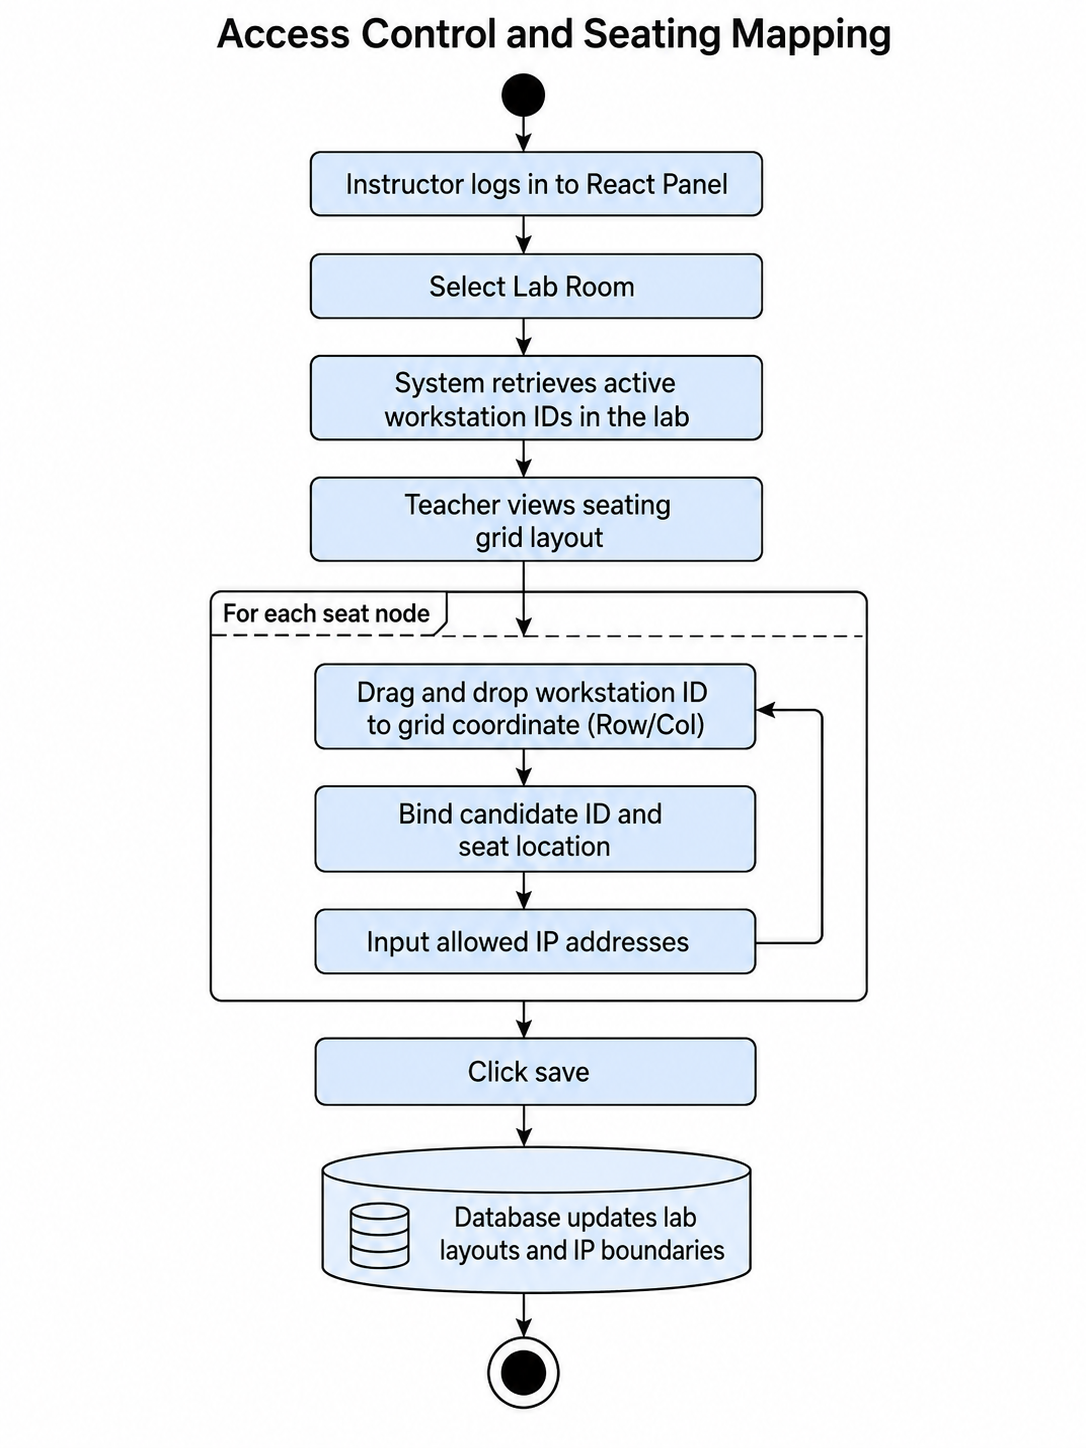
\includegraphics[width=0.97\linewidth]{Figures/activity_seating.png}
\caption{UML Activity Diagram of Access Control and Seating Mapping}
\label{fig:activity_seating}
\end{figure}

Teachers bind candidates to specific labs, IP addresses, and seat numbers to prevent remote logins.

\subsubsection{Live Dashboard Monitoring}
Figure~\ref{fig:activity_monitoring} outlines the real-time proctoring flow.

\begin{figure}[H]
\centering
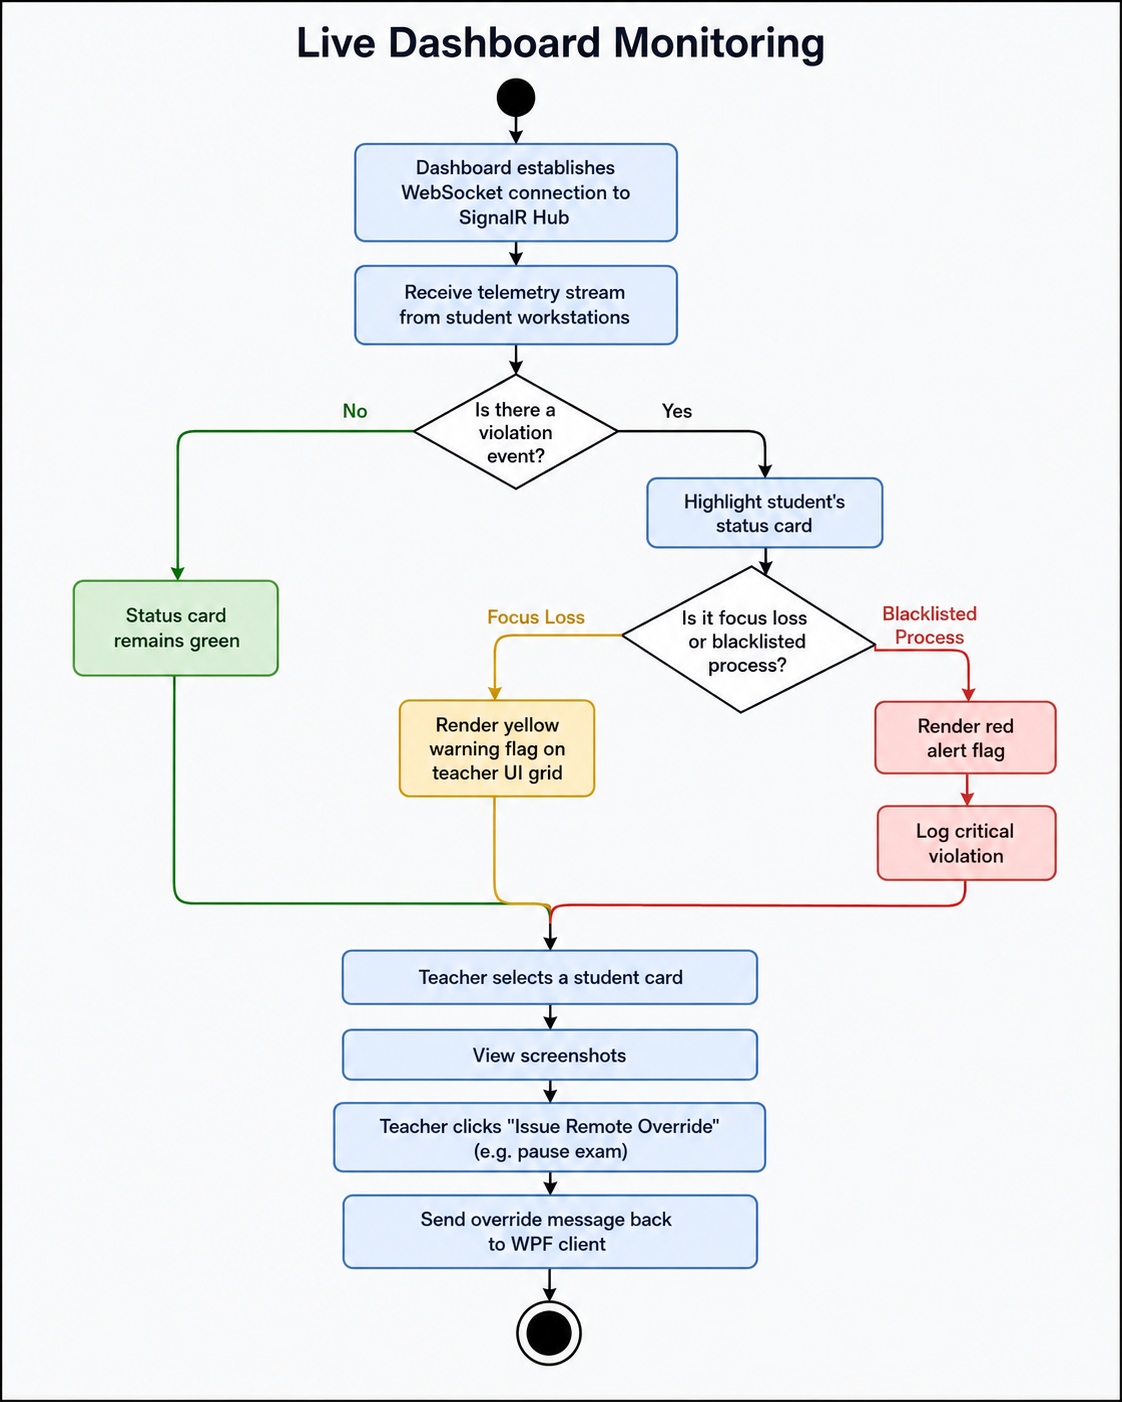
\includegraphics[width=0.97\linewidth]{Figures/activity_monitoring.png}
\caption{UML Activity Diagram of Live Dashboard Monitoring}
\label{fig:activity_monitoring}
\end{figure}

The React panel opens a WebSockets channel. It processes telemetry events, updating status cards and showing alerts if lock violations occur.

\subsubsection{AI-Assisted Grading and Similarity Check}
Figure~\ref{fig:activity_grading} maps post-exam grading.

\begin{figure}[H]
\centering
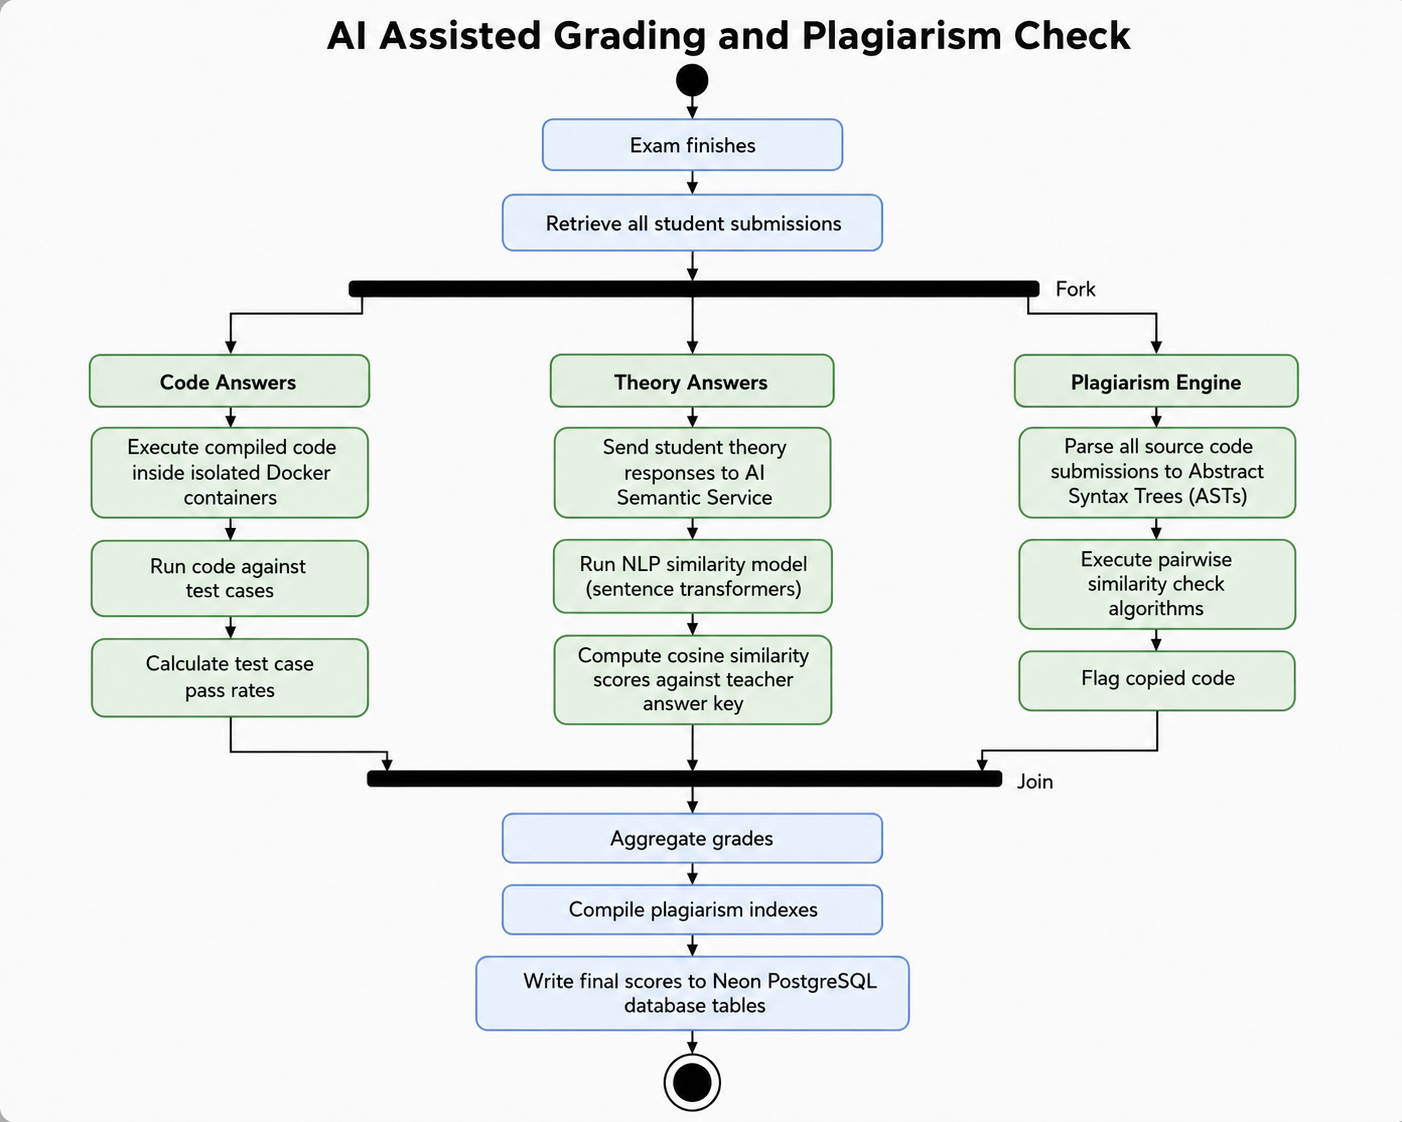
\includegraphics[width=0.97\linewidth]{Figures/activity_grading.png}
\caption{UML Activity Diagram of AI-Assisted Grading and Plagiarism Checking}
\label{fig:activity_grading}
\end{figure}

The engine executes student code inside isolated Docker environments to check against test cases, grades theory answers using NLP similarity, and runs AST comparisons to flag plagiarism.

\subsubsection{QuestPDF Report Generation}
Figure~\ref{fig:activity_report} shows the PDF rendering workflow.

\begin{figure}[H]
\centering
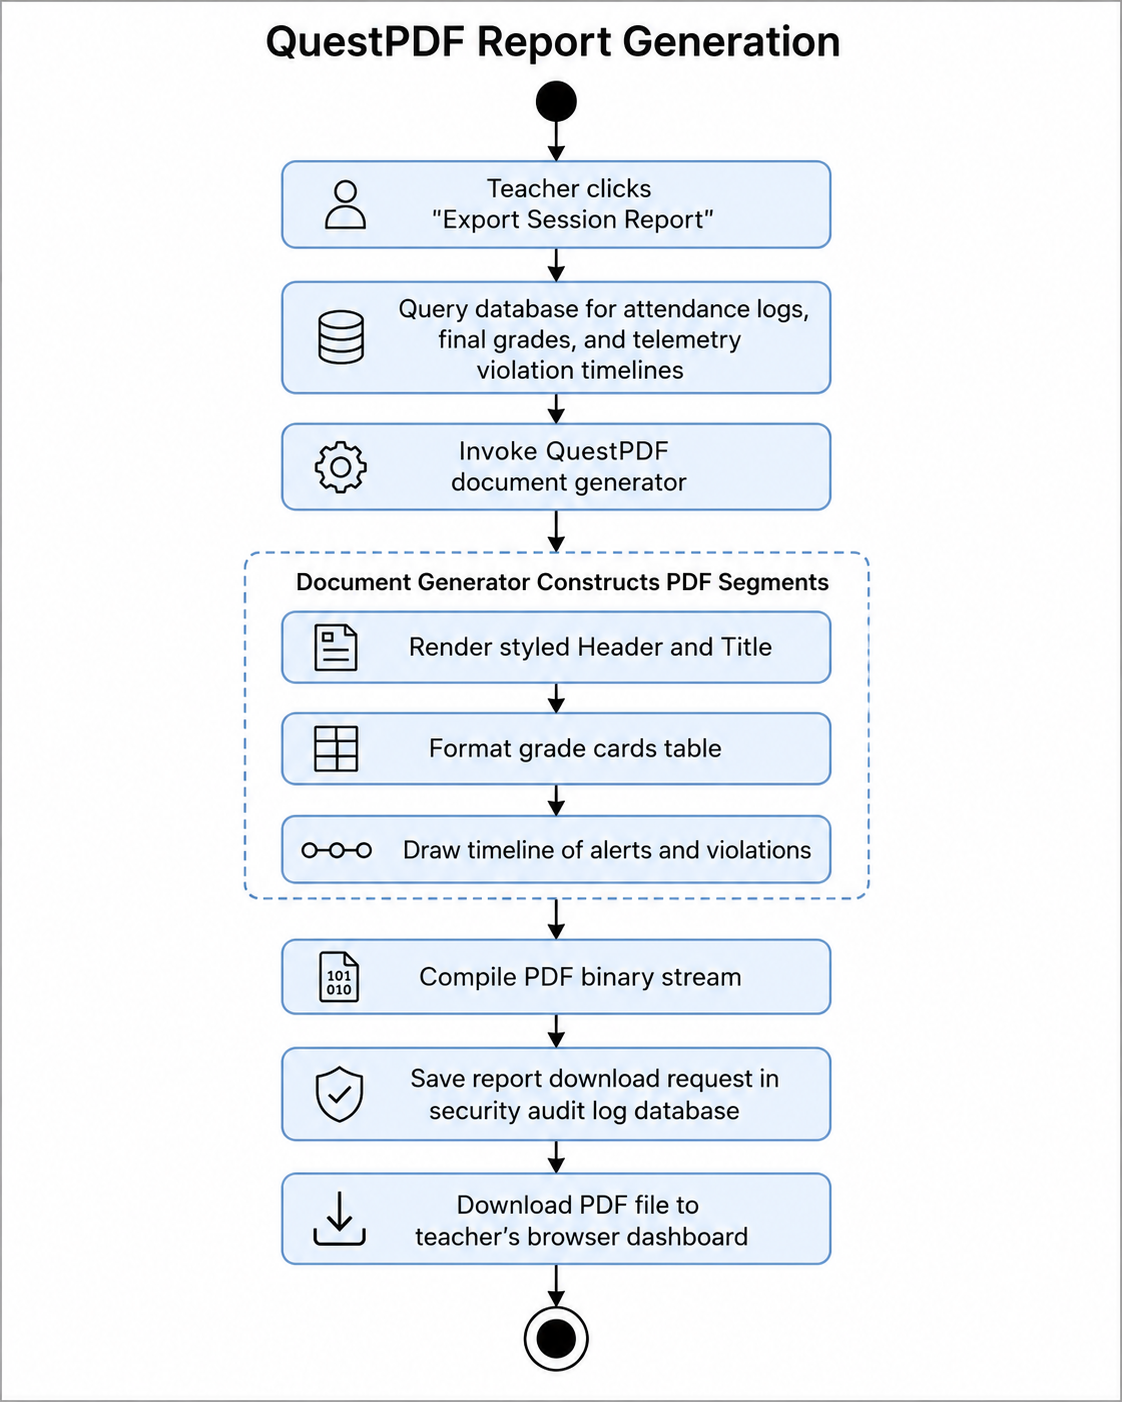
\includegraphics[width=0.97\linewidth]{Figures/activity_report.png}
\caption{UML Activity Diagram of QuestPDF Report Generation}
\label{fig:activity_report}
\end{figure}

The system compiles session metrics, formats the pages using QuestPDF, and downloads the PDF report.

\subsubsection{Audit Logging}
Figure~\ref{fig:activity_audit} details database auditing.

\begin{figure}[H]
\centering
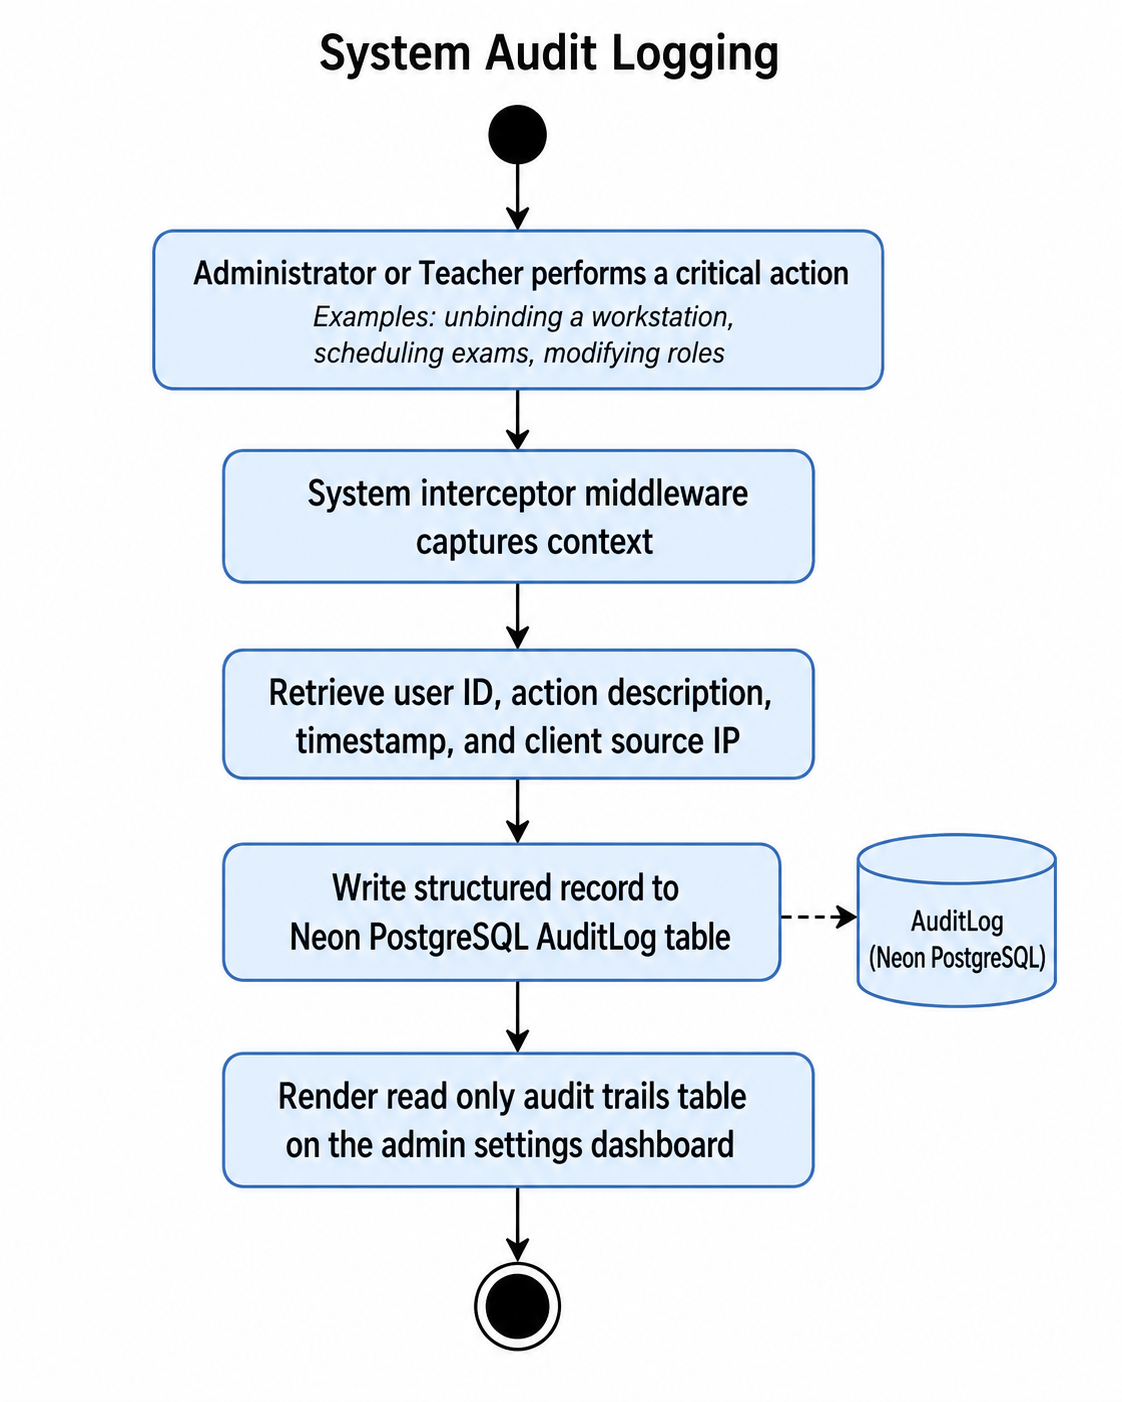
\includegraphics[width=0.97\linewidth]{Figures/activity_audit.png}
\caption{UML Activity Diagram of System Audit Logging}
\label{fig:activity_audit}
\end{figure}

Critical actions, such as seating overrides or password changes, are recorded in the database with timestamps and actor details.

\subsection{Communication Diagrams}
When focus-loss is identified at the client, there is a sequence of checks and processes that is completed to both alert and disable the client until a teacher overrides the lockdown \cite{communication_diagram_boardmix}. Figure~\ref{fig:communication_diagram} demonstrates the student override sequence in the system.

\begin{figure}[H]
\centering
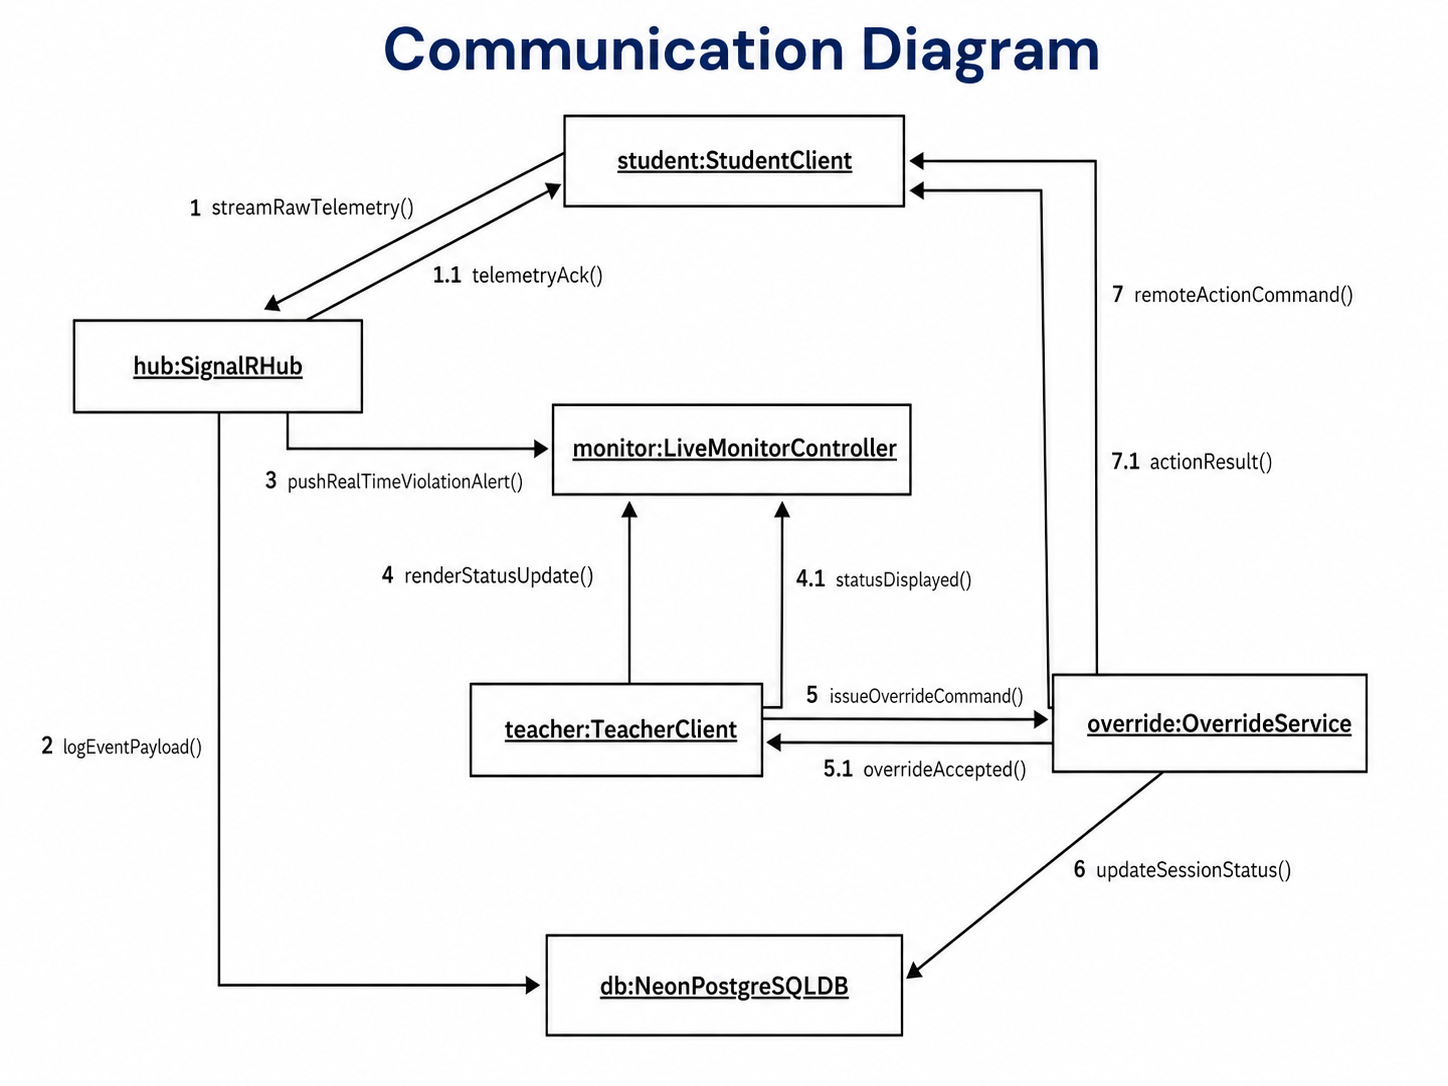
\includegraphics[width=0.97\linewidth]{Figures/communication_diagram.png}
\caption{UML Communication Diagram of real-time Telemetry Alerting and Teacher Overrides}
\label{fig:communication_diagram}
\end{figure}

Figure~\ref{fig:communication_diagram} maps the override sequence. The student client pushes a focus-loss event over WebSockets (1). The SignalR hub writes it to the database (2) and alerts the teacher panel (3). The teacher pauses the exam (4), sending an API call to the controller (5). The controller updates the database session (6) and instructs the hub to pause the student client (7).

\subsection{Sequence Diagrams}
A sequence diagram depicts when an object sends an information message, to whom it sends the information, the medium through which the information is sent, and how the objects interacting as part of the message send and receive in the form of time sequencing \cite{sequence_diagram_medium}. Figure~\ref{fig:seq_login} maps message sequences from student to login server.

\subsubsection{Login}
Figure~\ref{fig:seq_login} provides more details of the Login flow as explained above. Figure~\ref{fig:seq_login} maps message sequences from student to login server.

\begin{figure}[H]
\centering
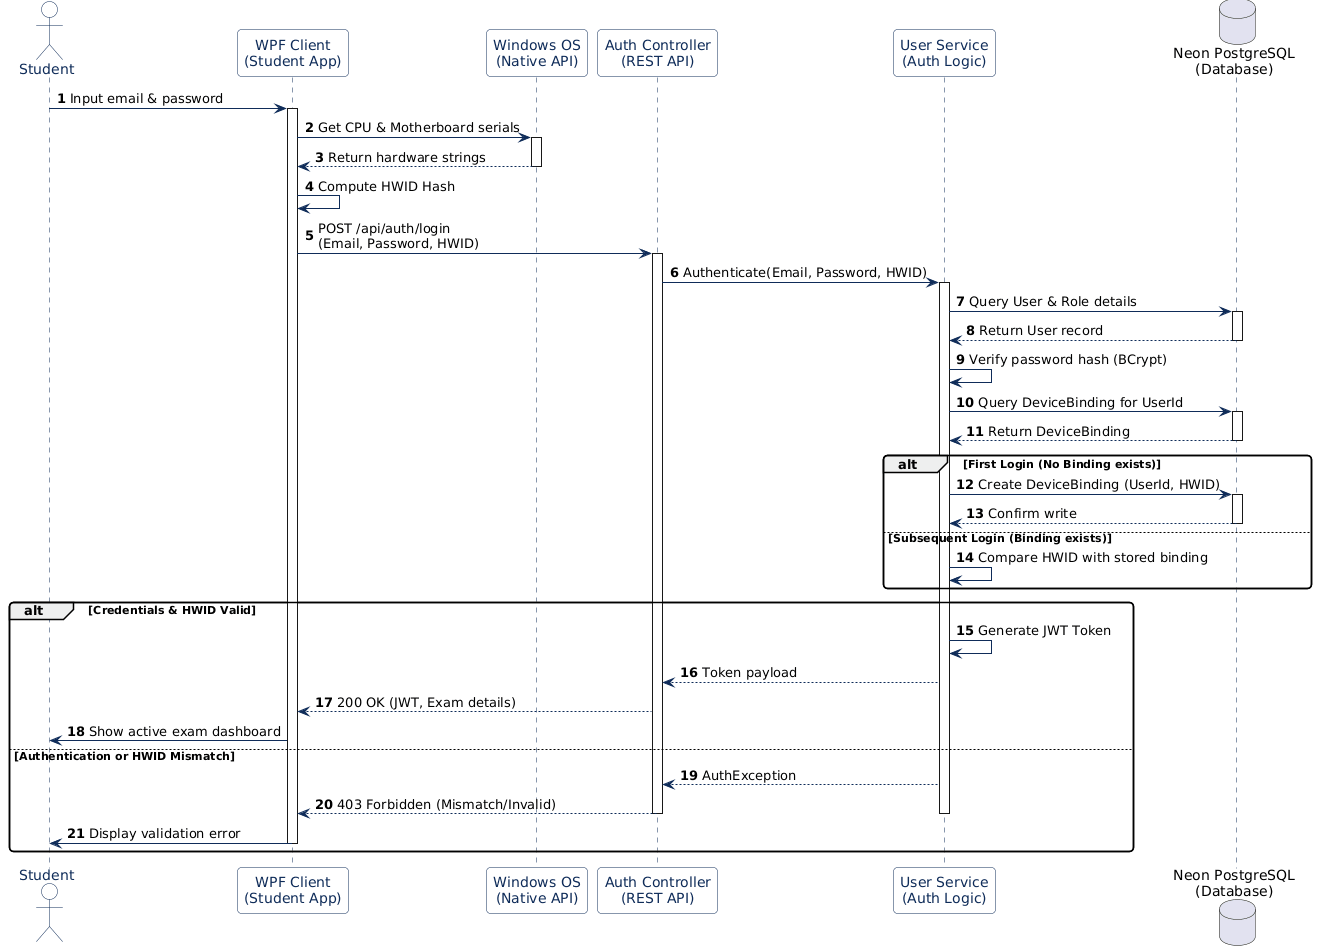
\includegraphics[width=0.97\linewidth]{Figures/seq_login.png}
\caption{Sequence Diagram of Student Login and HWID Verification}
\label{fig:seq_login}
\end{figure}

The student logs in on the WPF client. The client queries CPU and motherboard properties using native calls and transmits the hashed HWID to the server. The server compares this HWID with existing bindings. If matched, it returns a JWT; if mismatched, it blocks access.

\subsubsection{Logout}
Figure~\ref{fig:seq_logout} details logout.

\begin{figure}[H]
\centering
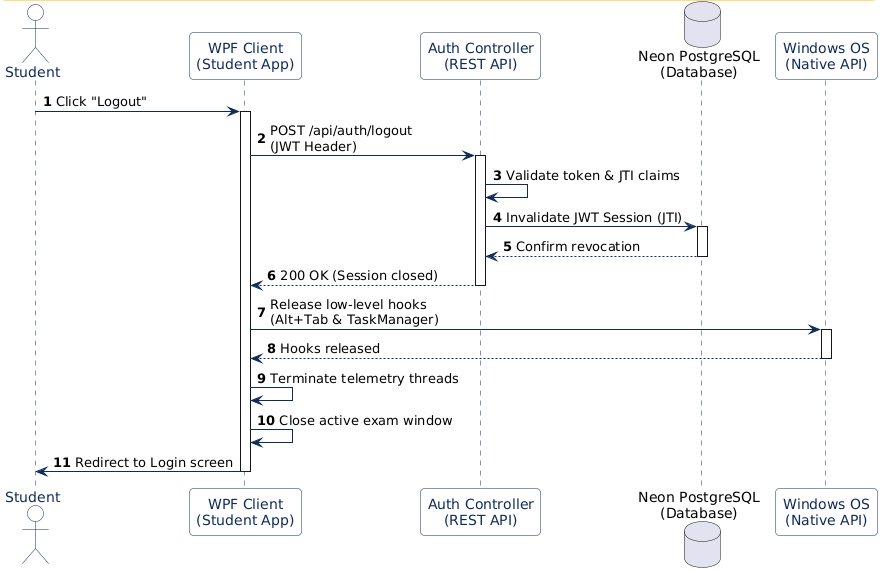
\includegraphics[width=0.97\linewidth]{Figures/seq_logout.png}
\caption{Sequence Diagram of Session Termination and Client Release}
\label{fig:seq_logout}
\end{figure}

The student requests logout. The server invalidates the active JWT session. On success, the client releases Windows hooks, stops telemetry threads, and returns the workstation to its default state.

\subsubsection{Change Password}
Figure~\ref{fig:seq_change_password} shows password modification.

\begin{figure}[H]
\centering
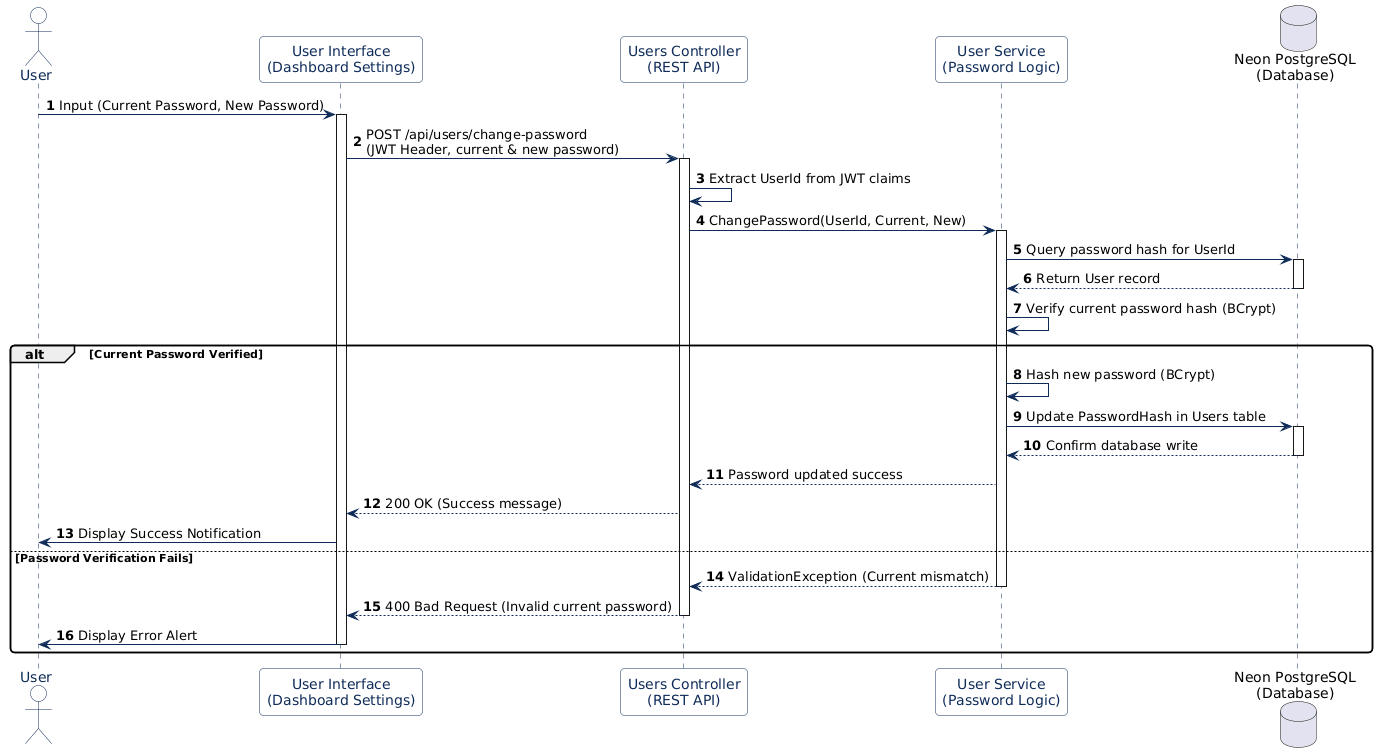
\includegraphics[width=0.97\linewidth]{Figures/seq_change_password.png}
\caption{Sequence Diagram of User Password Modification}
\label{fig:seq_change_password}
\end{figure}

The user submits credentials. The controller verifies their existing password using BCrypt, hashes the new password, and saves the update to PostgreSQL.

\subsubsection{View Database}
Figure~\ref{fig:seq_view_database} shows query flows.

\begin{figure}[H]
\centering
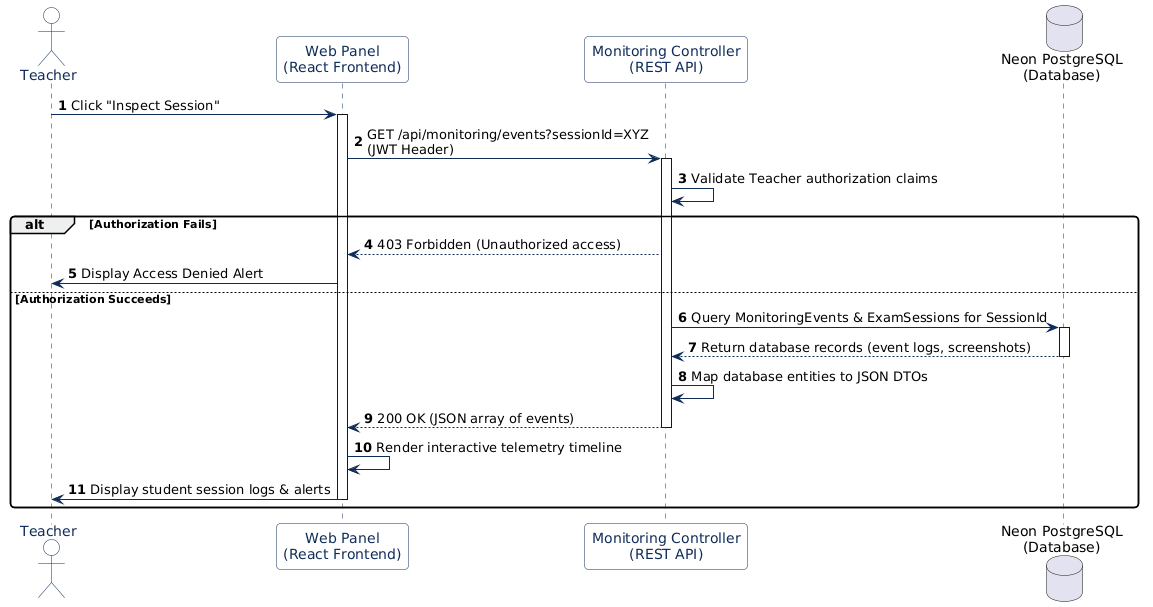
\includegraphics[width=0.97\linewidth]{Figures/seq_view_database.png}
\caption{Sequence Diagram of Teacher Querying Telemetry Events and Exam Records}
\label{fig:seq_view_database}
\end{figure}

Teachers request logs. The REST API validates teacher authorization, fetches telemetry records, formats them as a JSON list, and returns them to the React grid.

\subsubsection{Start Exam and Telemetry Ingestion}
Figure~\ref{fig:seq_telemetry} tracks telemetry loops.

\begin{figure}[H]
\centering
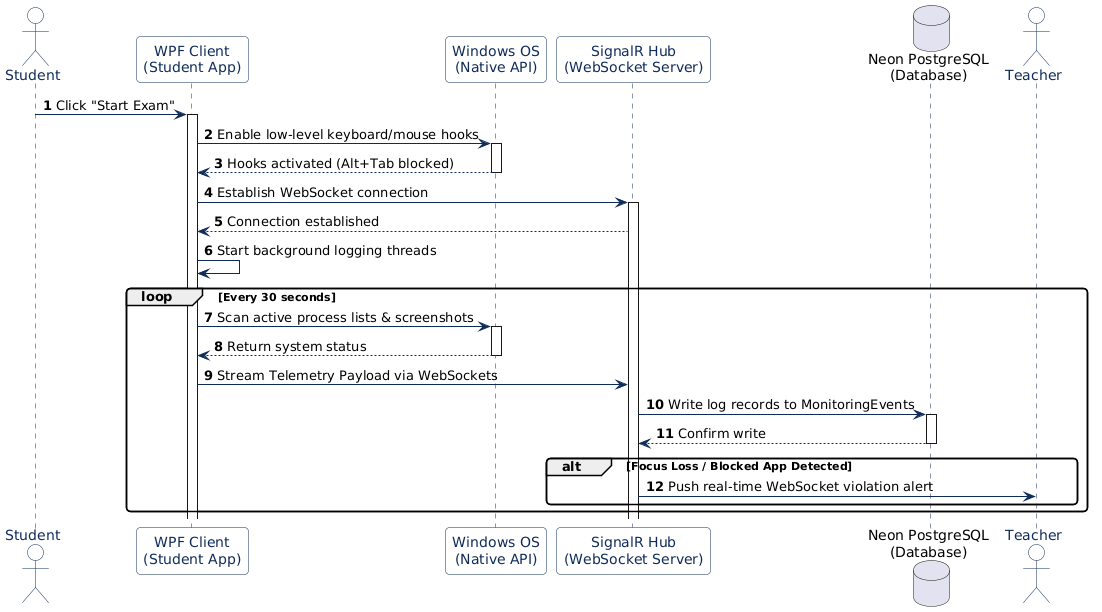
\includegraphics[width=0.97\linewidth]{Figures/seq_telemetry.png}
\caption{Sequence Diagram of Exam Launch and Background Telemetry Ingestion}
\label{fig:seq_telemetry}
\end{figure}

Launching the exam triggers native OS locks. The WPF client opens a WebSocket channel to the SignalR hub. Every 30 seconds, it queries OS handles and screenshot buffers, streaming them to the hub. The hub writes logs to Neon PostgreSQL and pushes warnings to the teacher if anomalies occur.

\subsubsection{Docker Code Compilation}
Figure~\ref{fig:seq_compilation} tracks sandboxed grading.

\begin{figure}[H]
\centering
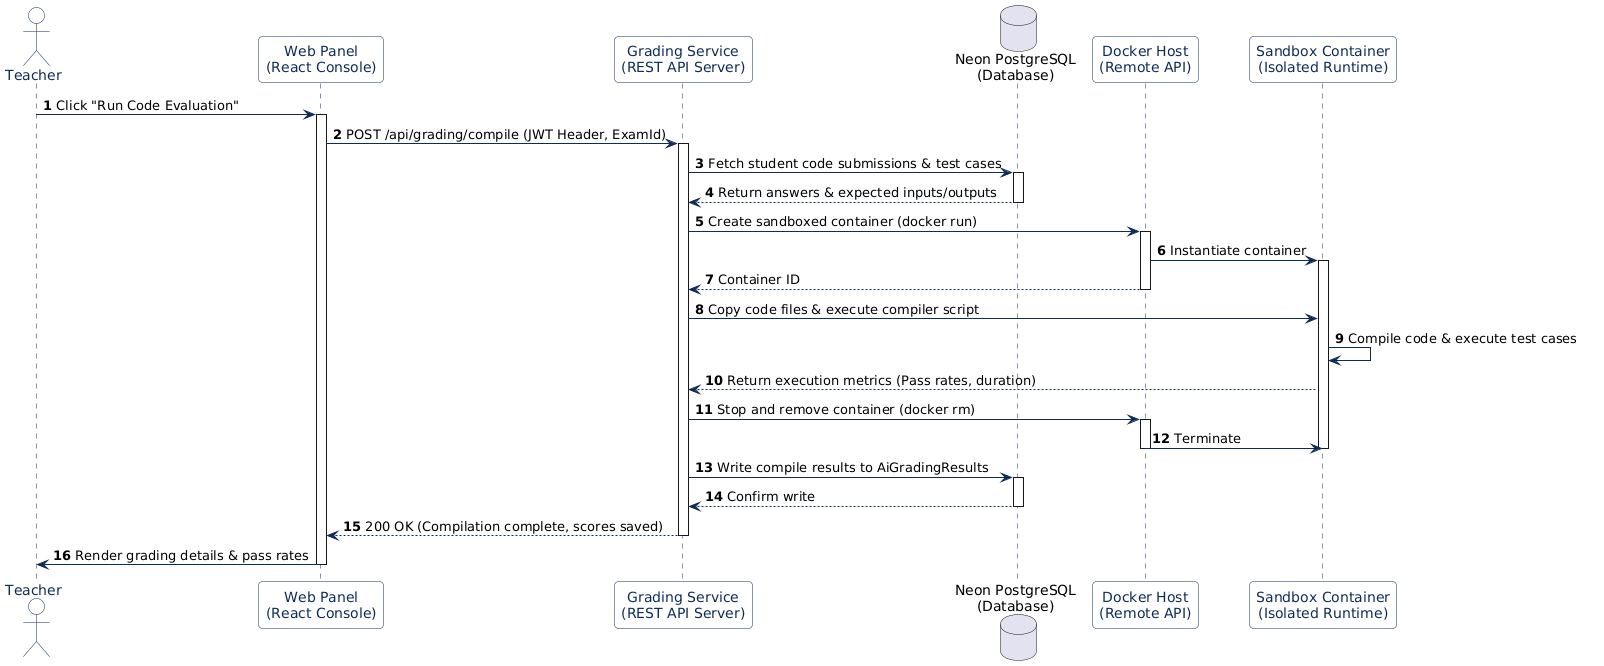
\includegraphics[width=0.97\linewidth]{Figures/seq_compilation.png}
\caption{Sequence Diagram of Isolated Code Compilation and Evaluation}
\label{fig:seq_compilation}
\end{figure}

When grading begins, the server fetches student code and test cases. It spins up a sandboxed Docker container, executes the compiler wrapper script inside, measures test execution metrics, stops the container, and logs scores in database.

\subsubsection{AI Semantic Grading and Plagiarism Check}
Figure~\ref{fig:seq_ai_plagiarism} shows AI and similarity checks.

\begin{figure}[H]
\centering
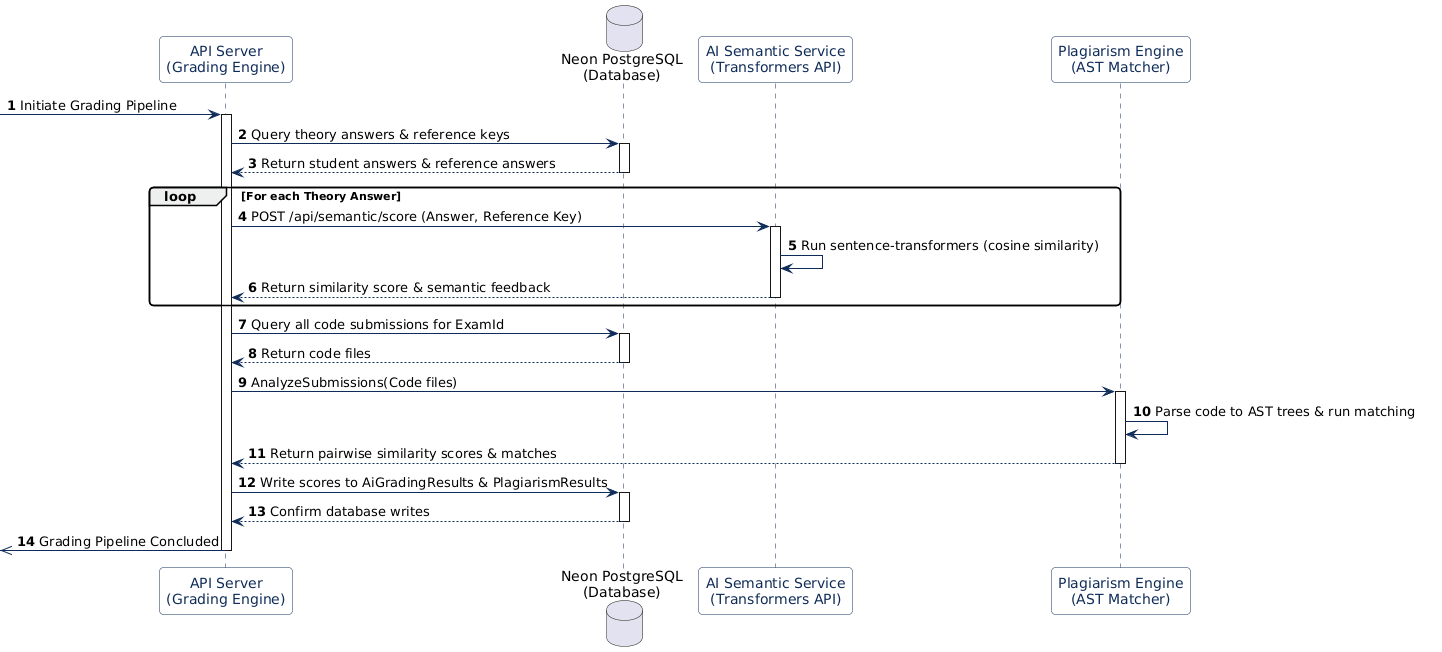
\includegraphics[width=0.97\linewidth]{Figures/seq_ai_plagiarism.png}
\caption{Sequence Diagram of AI Theory Grading and Plagiarism Checking}
\label{fig:seq_ai_plagiarism}
\end{figure}

The server queries theory answers and reference keys, requesting evaluations from the AI Semantic Service over HTTP. Following this, the Plagiarism Engine parses code files into ASTs to run pairwise checks across all student code files.

\subsubsection{Pre-Exam Diagnostics Check}
Figure~\ref{fig:seq_diagnostics} outlines pre-exam hardware diagnostics.

\begin{figure}[H]
\centering
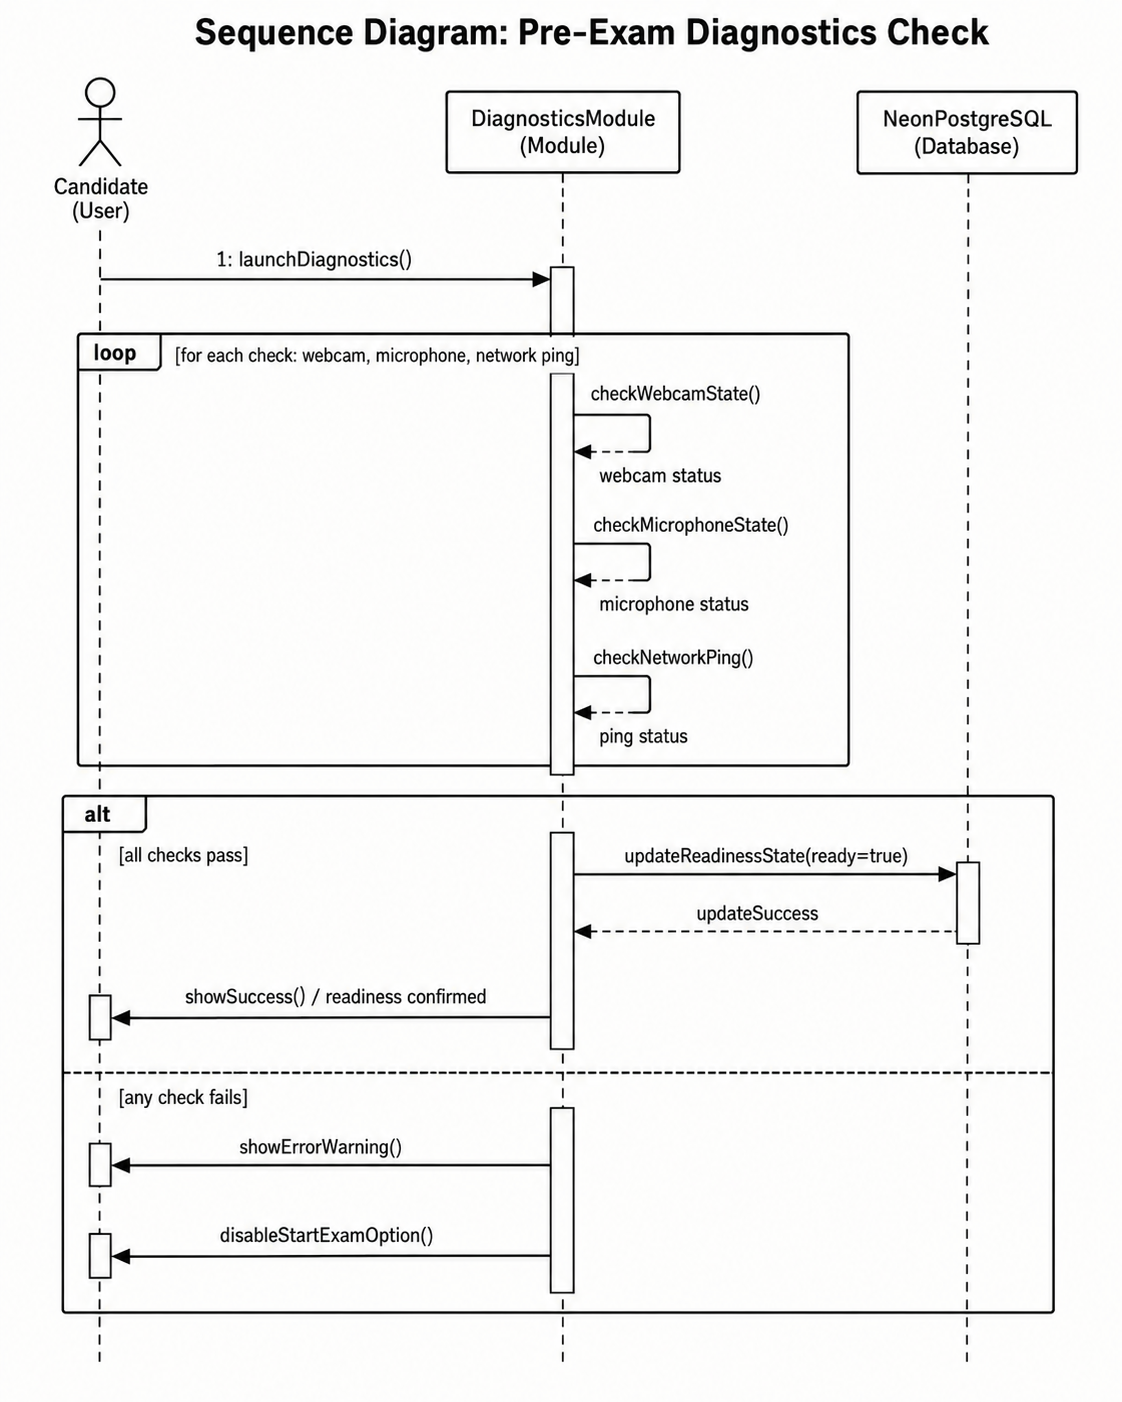
\includegraphics[width=0.97\linewidth]{Figures/seq_diagnostics.png}
\caption{Sequence Diagram of Pre-Exam Workstation Diagnostics Check}
\label{fig:seq_diagnostics}
\end{figure}

The client queries local hardware loops for webcam/mic states and tests internet latency. Success enables the proceed button, while failures trigger diagnostic warnings.

\subsubsection{Readiness Verification and Mock Test}
Figure~\ref{fig:seq_readiness} maps mock tests.

\begin{figure}[H]
\centering
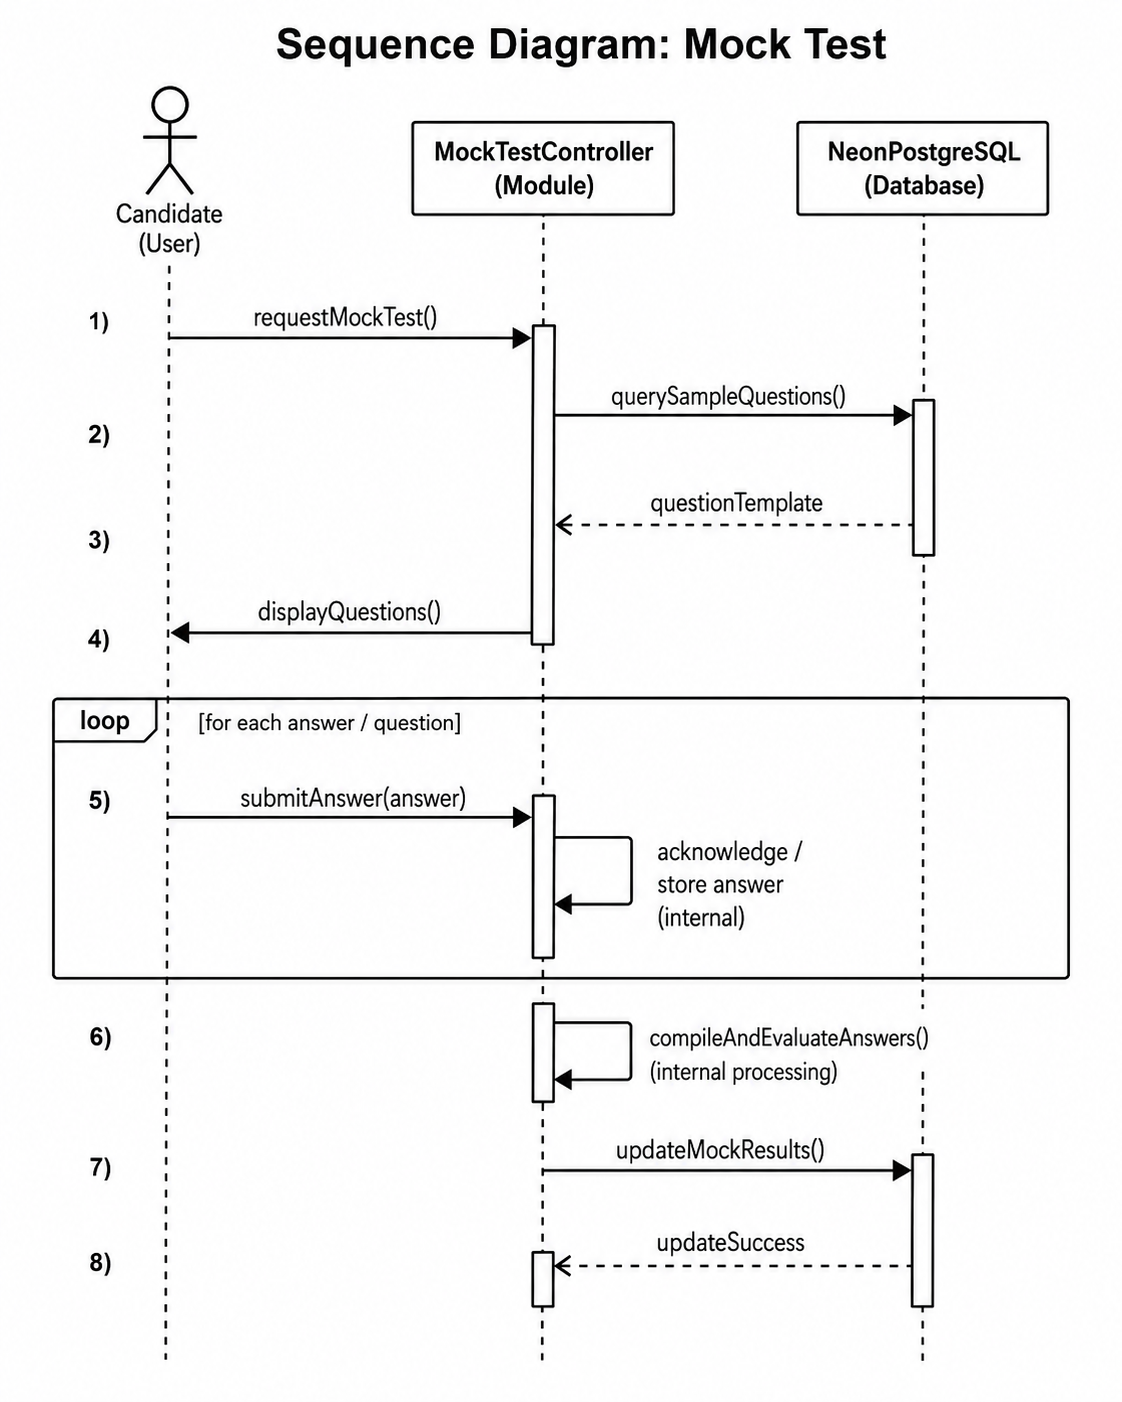
\includegraphics[width=0.97\linewidth]{Figures/seq_readiness.png}
\caption{Sequence Diagram of Readiness Verification and Mock Test}
\label{fig:seq_readiness}
\end{figure}

Students run a mock test. The client pulls questions, allows editing, compiles the mock submissions, and returns scores.

\subsubsection{Lockdown Mode Enforcement}
Figure~\ref{fig:seq_lockdown} details desktop lockdown.

\begin{figure}[H]
\centering
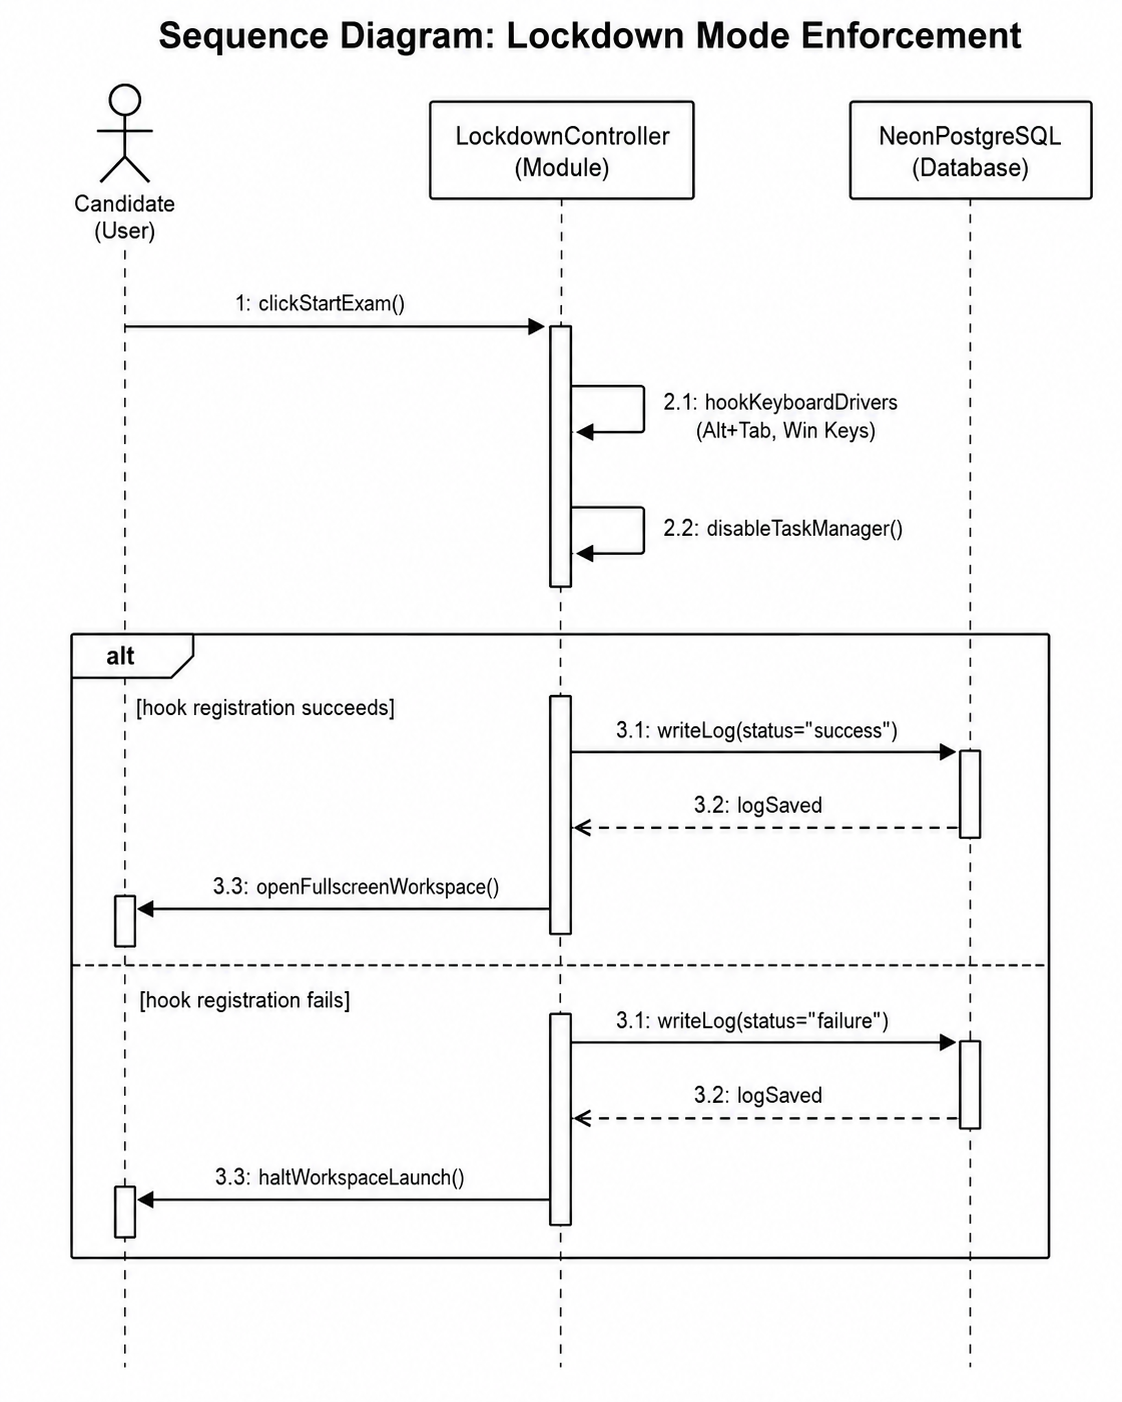
\includegraphics[width=0.97\linewidth]{Figures/seq_lockdown.png}
\caption{Sequence Diagram of Student Client Lockdown Mode Enforcement}
\label{fig:seq_lockdown}
\end{figure}

Starting the exam triggers hooks that disable key combinations (Alt+Tab, Win Key). The client writes lock success logs to Neon PostgreSQL and displays the fullscreen exam workspace.

\subsubsection{Auto-Save and Session Recovery}
Figure~\ref{fig:seq_recovery} tracks local recovery backups.

\begin{figure}[H]
\centering
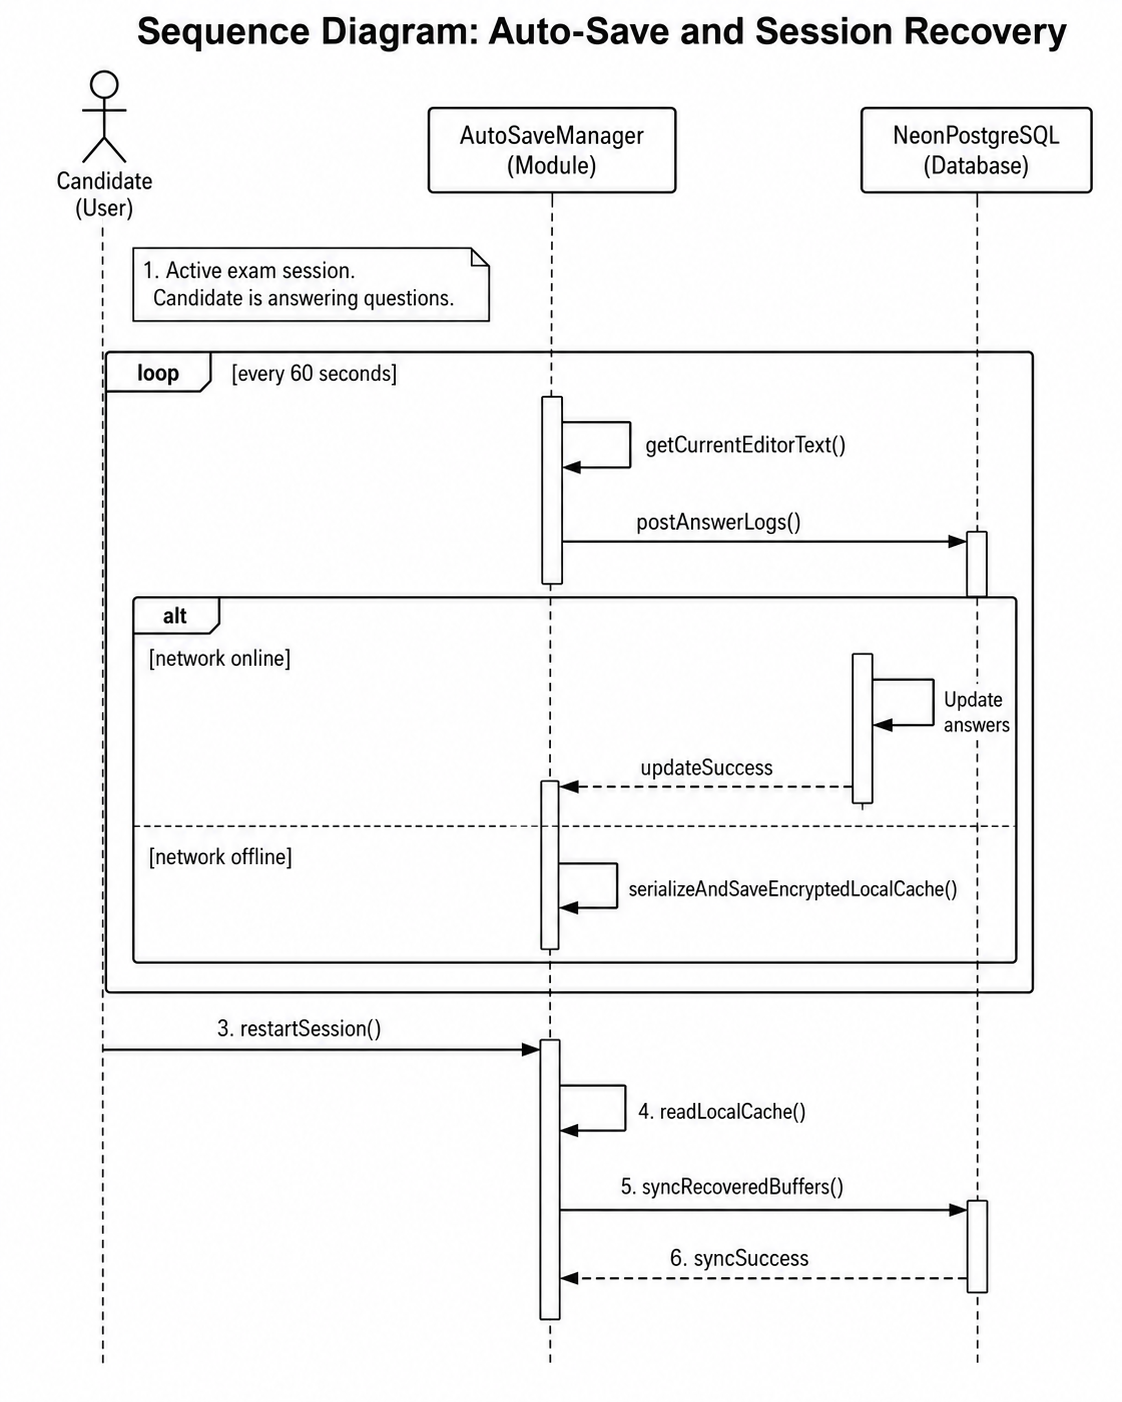
\includegraphics[width=0.97\linewidth]{Figures/seq_recovery.png}
\caption{Sequence Diagram of Auto-Save and Session Recovery}
\label{fig:seq_recovery}
\end{figure}

A 60-second loop collects editor changes. If offline, the client writes the backup to a local encrypted cache, which recovers and syncs when a network connection is re-established.

\subsubsection{Exam Submission (Controlled)}
Figure~\ref{fig:seq_submission} shows final submissions.

\begin{figure}[H]
\centering
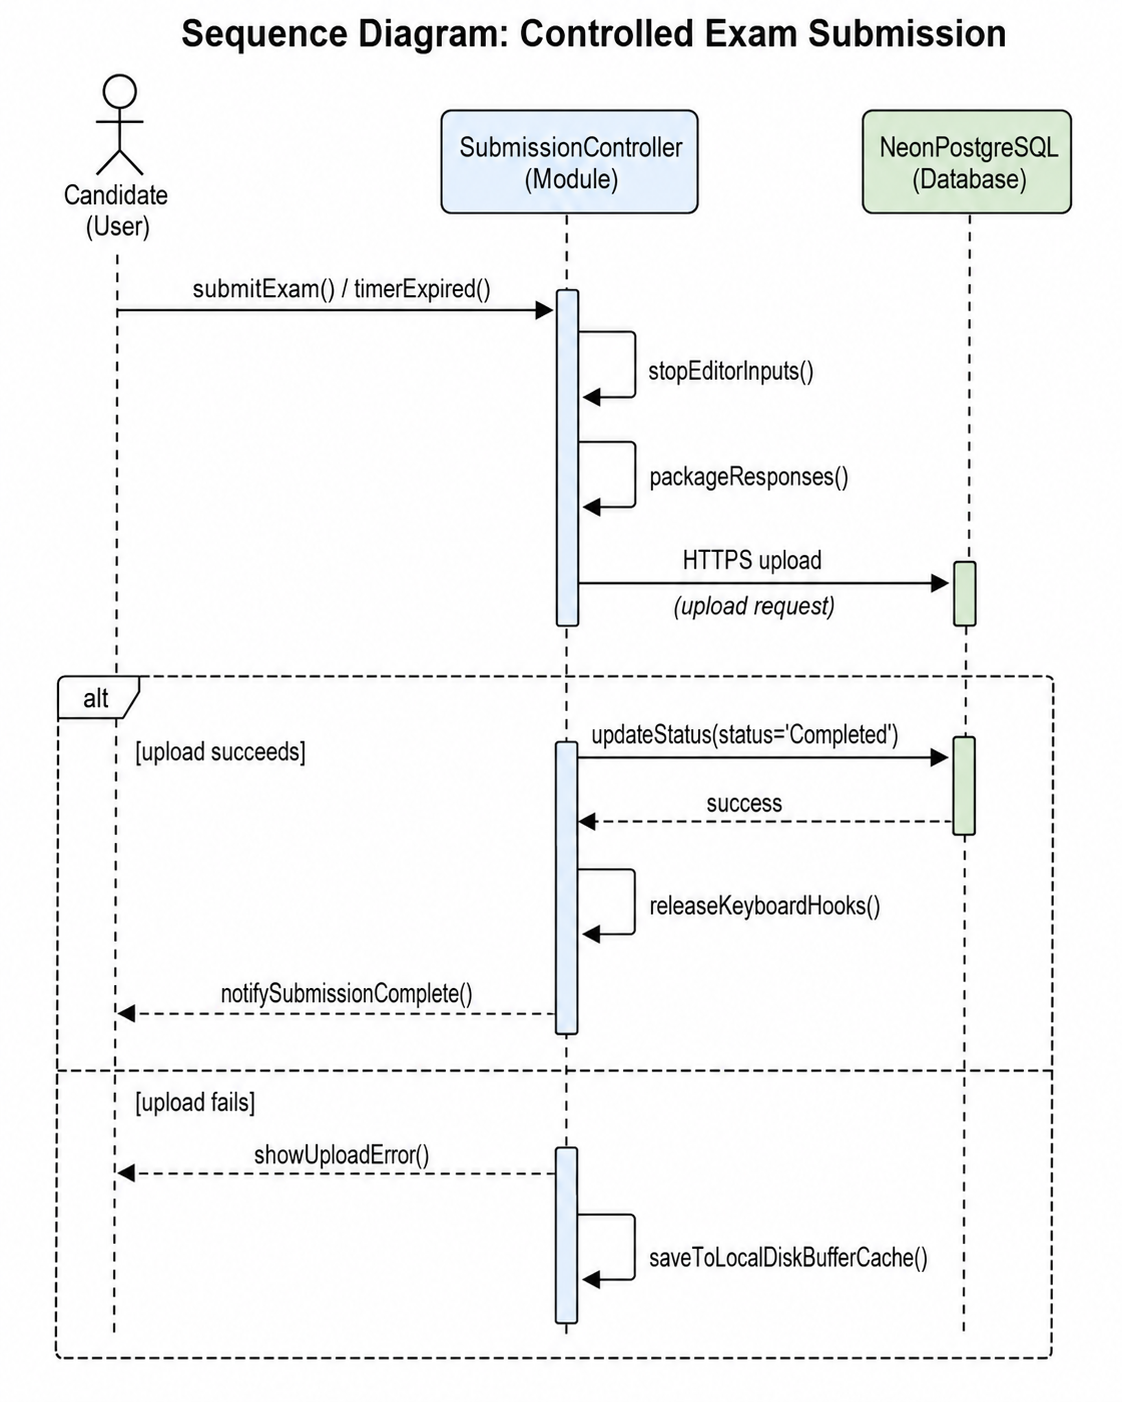
\includegraphics[width=0.97\linewidth]{Figures/seq_submission.png}
\caption{Sequence Diagram of Controlled Exam Submission}
\label{fig:seq_submission}
\end{figure}

The student submits their exam. The client locks inputs, bundles answers, uploads the payload over HTTPS, updates database session rows, and releases all keystroke hooks.

\subsubsection{Exam Template Configuration}
Figure~\ref{fig:seq_config} maps template creation.

\begin{figure}[H]
\centering
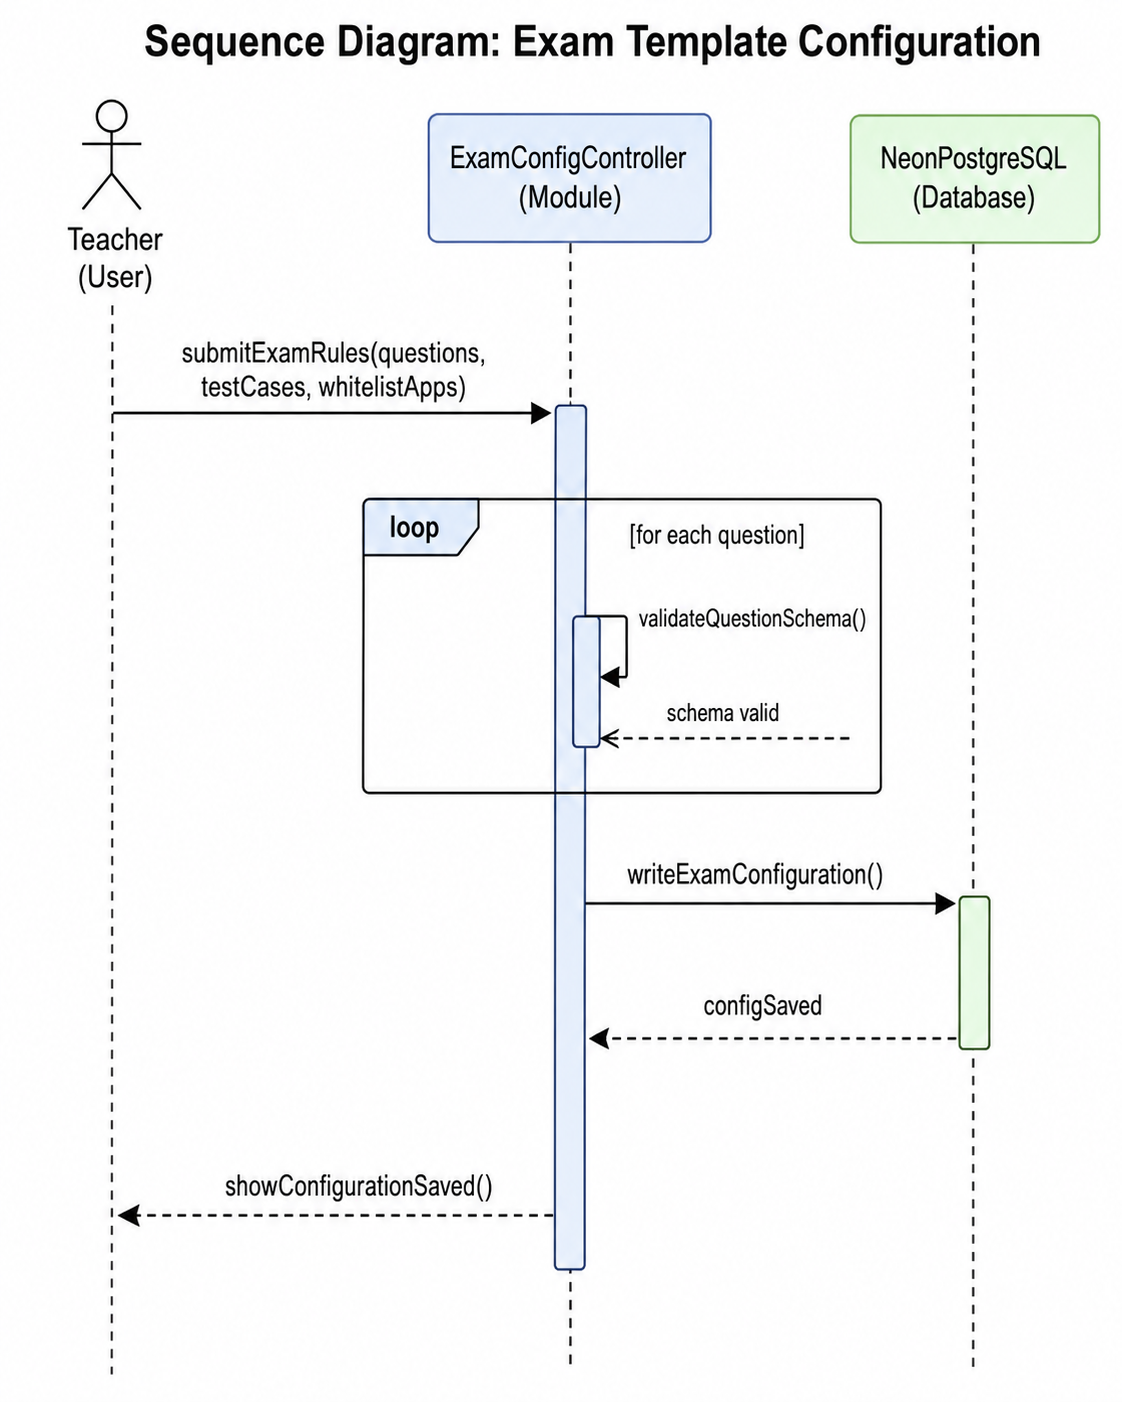
\includegraphics[width=0.97\linewidth]{Figures/seq_config.png}
\caption{Sequence Diagram of Exam Template Configuration}
\label{fig:seq_config}
\end{figure}

The React panel sends config metadata (durations, whitelisted apps, test cases) to the API. The API verifies the details, updates the database, and returns confirmation.

\subsubsection{Audit Logging and Report Export}
Figure~\ref{fig:seq_audit} shows reporting sequence.

\begin{figure}[H]
\centering
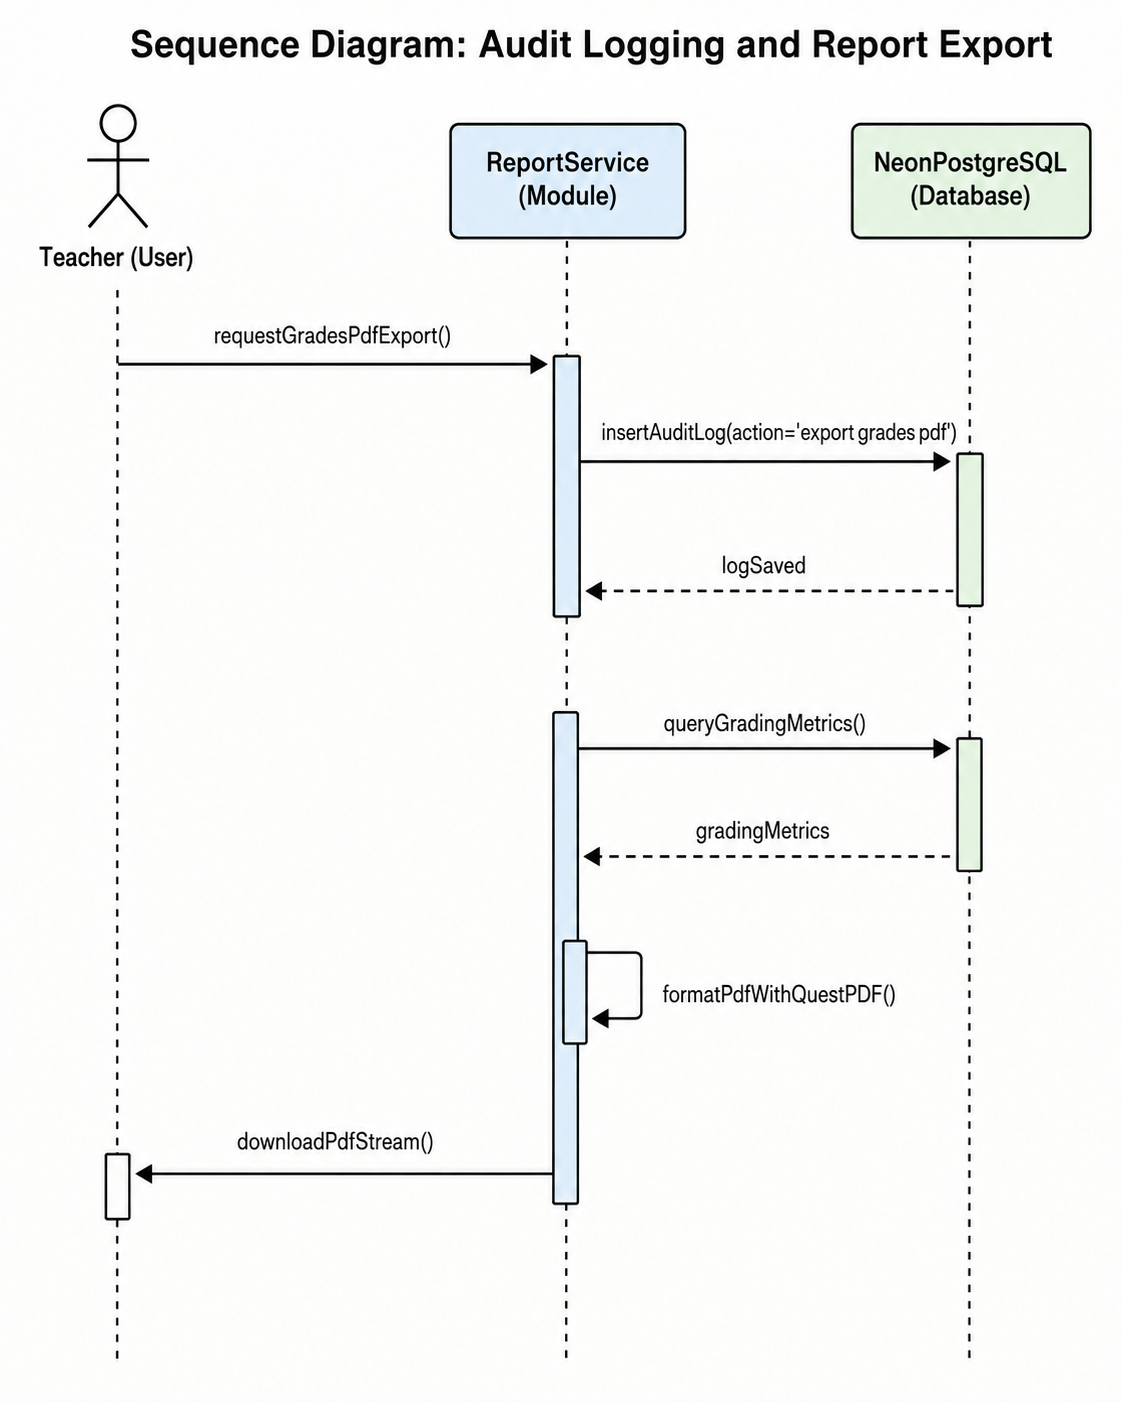
\includegraphics[width=0.97\linewidth]{Figures/seq_audit.png}
\caption{Sequence Diagram of Audit Logging and Report Export}
\label{fig:seq_audit}
\end{figure}

Teachers request reports. The REST API logs the request in audit tables, pulls grading summaries, calls QuestPDF to build the layout, and streams the PDF document to the browser.